\documentclass{article}
\usepackage{fontenc}
\usepackage[ngerman]{babel}
\usepackage[utf8]{inputenc}
\usepackage{graphicx}
\usepackage{grffile}
\usepackage{subcaption}
\usepackage[export]{adjustbox}
\graphicspath{ {../pics/Blatt 2} }
\usepackage{alphalph}
\DeclareUnicodeCharacter{2028}{\linebreak}
\usepackage{hyperref}
\usepackage{listings}
\usepackage{color}

\definecolor{dkgreen}{rgb}{0,0.6,0}
\definecolor{gray}{rgb}{0.5,0.5,0.5}
\definecolor{mauve}{rgb}{0.58,0,0.82}

\lstset{frame=tb,
  language=Java,
  aboveskip=3mm,
  belowskip=3mm,
  showstringspaces=false,
  columns=flexible,
  basicstyle={\small\ttfamily},
  numbers=left,
  numberstyle=\tiny\color{gray},
  keywordstyle=\color{blue},
  commentstyle=\color{dkgreen},
  stringstyle=\color{mauve},
  breaklines=true,
  breakatwhitespace=true,
  tabsize=3
}
\usepackage{datetime}
\newdateformat{myformat}{\THEDAY{ten }\monthname[\THEMONTH], \THEYEAR}

\begin{document}
	\begin{titlepage}
		\centering
		{\scshape\LARGE
			Ereignisdiskrete Systeme
			\par}
		\vspace{1.5cm}
		{\huge\bfseries Praktikum Blatt 2 - Simulink\par}
		\vspace{1.5cm}
		{\LARGE\itshape Jan Kristel, Alexandra Moritz\par}
		\vfill
			Aufsicht von Frau Rembold\par
			
		\vfill	
			{\large \today \par}	
		
	\end{titlepage}
	
	\tableofcontents
	\newpage
	
	\section{Grundlagen}
		\subsection{Welcher Übertragungstyp?}
			\renewcommand{\thesubsubsection}{\alph{subsubsection})}
			\subsubsection{}
				$$h_1(t) = \frac{\frac{1}{4}}{s}$$
				Es handelt sich um die Sprungfunktion eines I-Glied
			\subsubsection{}
				$$h_2(t) = \frac{s}{s + 1}$$
				Die Sprungfunktion ist von einem $DT_1$-Glied.
			\subsubsection{}
				$$h_3(t) = \frac{2}{0,95s^2 + 0,19s +1}$$
				Das Bild zeigt die Sprungfunktion eines $PT_2$-Glieds an.
			\subsubsection{}
				$$h_4(t) = \frac{1}{s + 1}$$
				Hierbei sieht man den Graphen der Sprungfunktion eines verzögerten $PT_1$-Glieds.
		\subsection{Relevante Parameter}
			\subsubsection{}
				\begin{itemize}
					\item $K_I = \frac{1}{4} \rightarrow$ dient der Steigung. Dies lässt sich aus dem Bild/Graph ablesen.
				\end{itemize}
			\subsubsection{}
				\begin{itemize}
					\item $K_D = \frac{1}{1} = 1$. Dies sorgt für ein bestehendes $s$ im Zähler.
					\item $T_1 = 1$, was für ein vorhandenes $s$ im Nenner sorgt.
				\end{itemize}
			\subsubsection{}
				\begin{itemize}
					\item $K_P = 2$, durch ablesen bestimmt.
					\item $T_2$ und $T_1$ müssen berechnet werden:
						\begin{itemize}
							\item $$\vartheta  = ln\Big(\frac{\Delta_1}{\Delta_2} \Big) = ln \Big(\frac{1,5}{1}\Big) = 0,3$$ $\rightarrow \Delta_1 und \Delta_2$ sind die ersten beiden Schwingungen der Sprungfunktion, nachdem diese den $K_P = 2$ gekreuzt haben.
							\item $$d = \frac{\vartheta}{\sqrt{\pi^2 + \vartheta^2}} = \frac{0,3}{\sqrt{\pi^2 + ^2}} = 0,098$$
							\item $$\omega_e = \frac{2\cdot \pi}{T_e} = \frac{2\cdot \pi}{6} = 1,047$$ $\rightarrow T_e$ lässt sich aus dem Graphen abschätzen. Das ist die Dauer für die ersten vollständige Schwingung nachdem $K_P$ erreicht wurde.
							\item $$\omega_0 = \frac{\omega_e}{\sqrt{1 - d^2}} = \frac{1,047}{\sqrt{1 - 0,098^2}} = 1,052$$ 
							\item $$T_2 = \frac{1}{\omega_0} = \frac{1}{1,052} = 0,95$$
							\item $$T_1 = 2\cdot d \cdot T_2 = 2 \cdot 0,098 \cdot 0,95 = 0,19$$
						\end{itemize}
				\end{itemize}
			\subsubsection{}
				\begin{itemize}
					\item $K_P = \frac{1}{1} = 1$ Dies lässt sich wieder aus dem Graph ablesen.
					\item $T_1 = 1$
					\item $t = 1 \rightarrow$ die Verzögerung $t$ lässt sich ablesen und in Simulink durch ein extra Verzögerungsglied einstellen.
				\end{itemize}
\newpage
		\subsection{Überprüfung durch Simulink}
			\subsubsection{}
				\begin{figure}[h]
					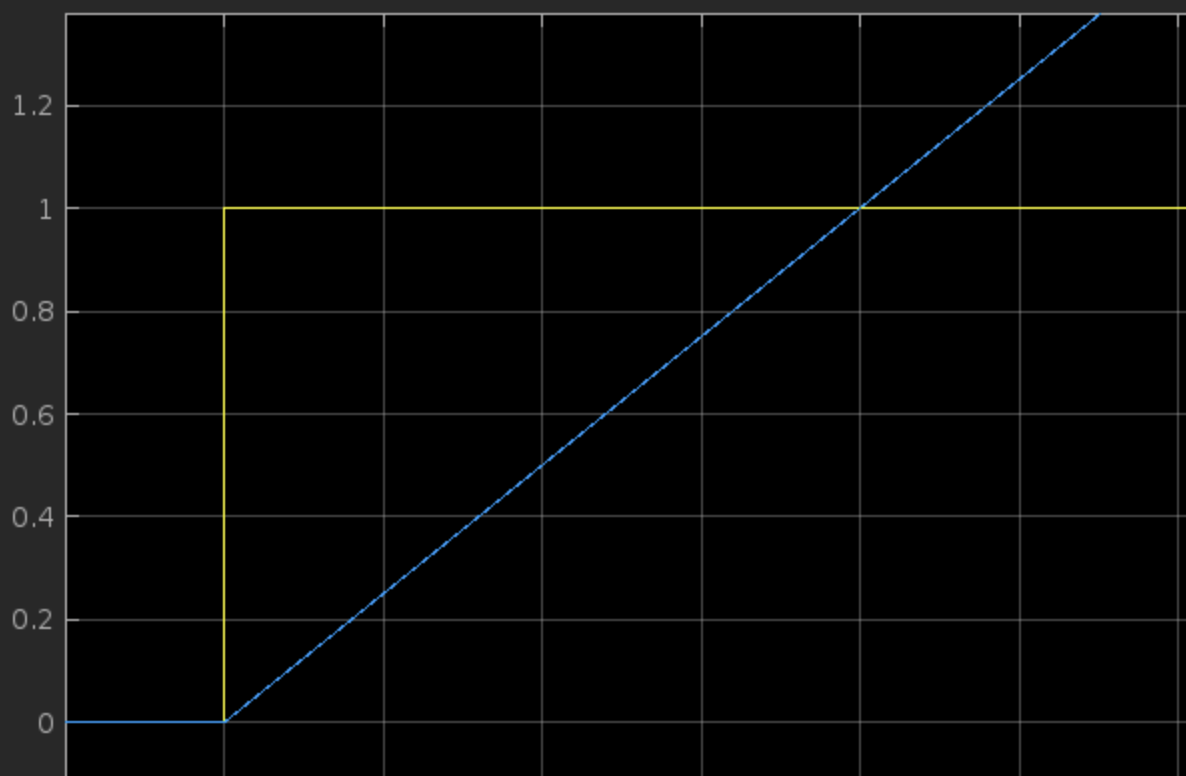
\includegraphics[scale=0.22, center]{./Sprungfunktion_I_Glied.png}
					\caption{Graph einer Sprungfunktion eines I-Glieds.}
					\label{fig1: Springfunktion-I-Glied}
				\end{figure}	
			\subsubsection{}
				\begin{figure}[h]
					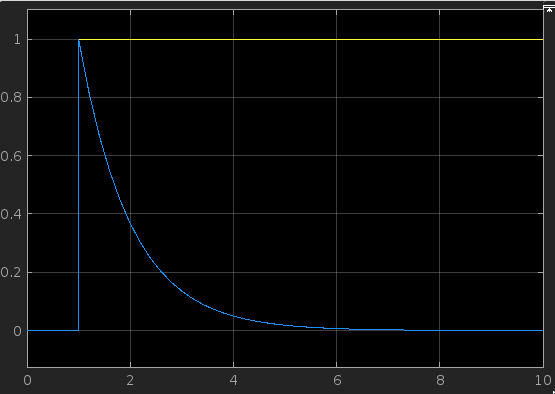
\includegraphics[scale=0.47, center]{./Sprungfunktion_DT_1_Glied.png}
					\caption{Graph einer Sprungfunktion eines $DT_1$-Glieds.}
					\label{fig2: Springfunktion-DT-1-Glied}
				\end{figure}	
\newpage
			\subsubsection{}
				\begin{figure}[ht]
					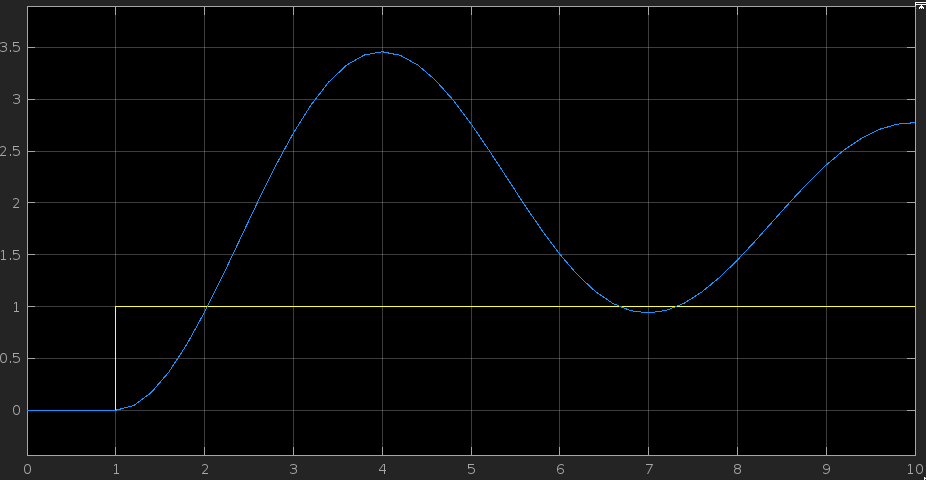
\includegraphics[scale=0.4, center]{./Sprungfunktion_PT_2_Glied.png}
					\caption{Graph einer Sprungfunktion eines $PT_2$-Glieds.}
					\label{fig3: Springfunktion-PT-2-Glied}
				\end{figure}	
			\subsubsection{}
				\begin{figure}[ht]
					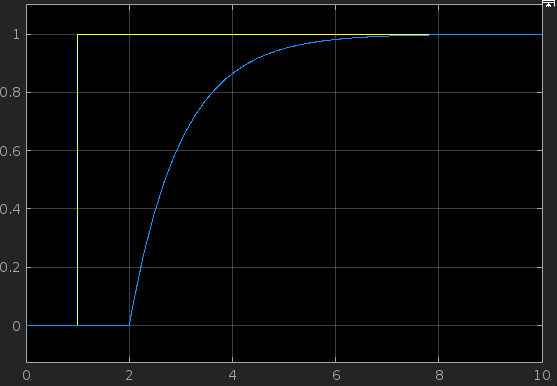
\includegraphics[scale=0.4, center]{./Sprungfunktion_PT_1_Glied_verzoegert.png}
					\caption{Graph einer Sprungfunktion eines um 1 Zeiteinheit verzögertes $PT_1$-Glieds.}
					\label{fig3: Springfunktion-PT-1-Glied}
				\end{figure}	
\newpage
	\section{Optimierung eines einfachen Regelkreises}
		\subsection{Übertragungsverhalten}
			Die Übertragsfunktion/Übertragungsverhalten für die Geschwindigkeit $v_x(t)$ lautet:
			$$G_u(s) = \frac{X(s)}{v_x(s)} = \frac{1}{s}$$
		
		\subsection{1.Näherung}
			\subsubsection{Lageregelkreis in Simulink}
				\begin{figure}[h]
					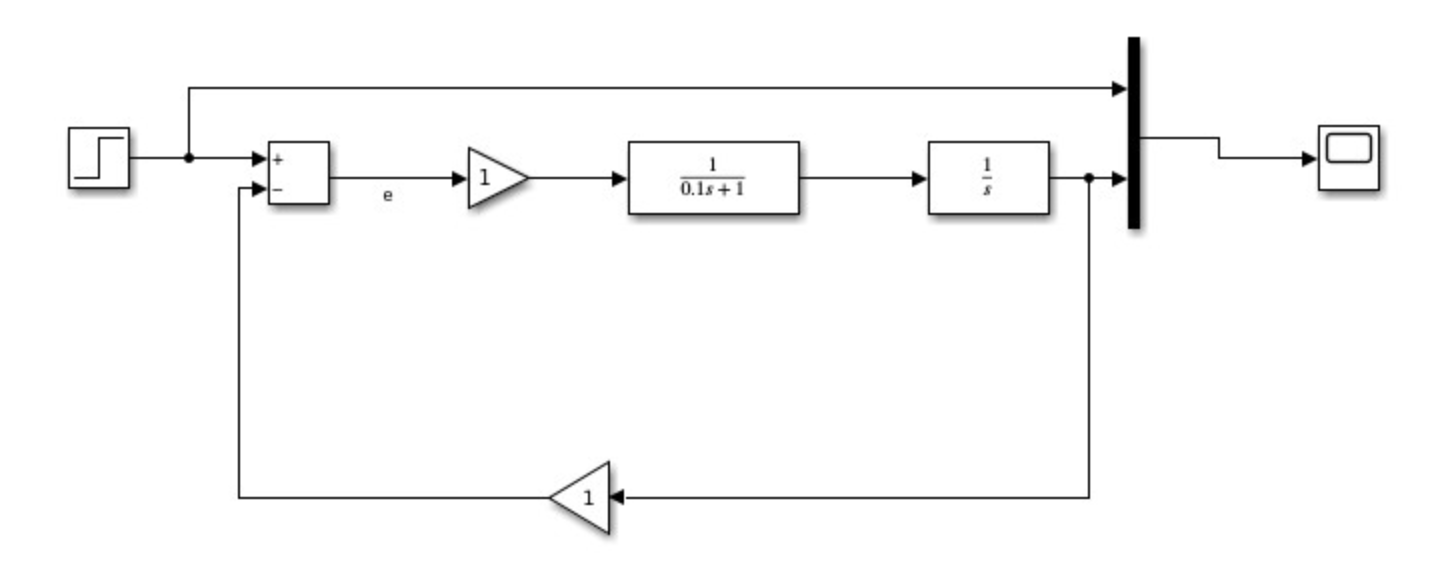
\includegraphics[scale=0.4, center]{2_b_1_Regelkreis.png}
					\caption{Aufbau des Regelkreises}
					\label{fig4: Lageregelkreis_b_1}
				\end{figure}
\newpage
			\subsubsection{Optimierung des Regelkreises - durch ausprobieren}
				\begin{figure}[h]
					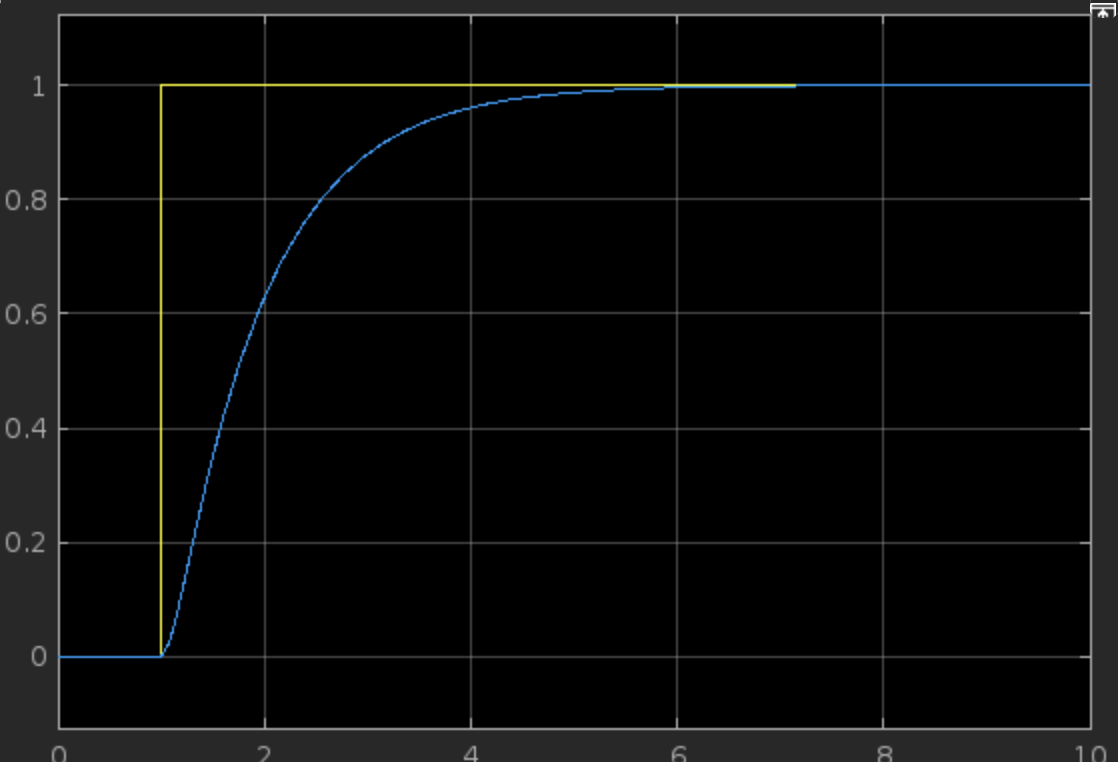
\includegraphics[scale=0.2325, center]{2_b_2_KP_1.png}
					\caption{$K_P = 1$}
					\label{fig5: Graph_KP_1}
				\end{figure}
				\begin{figure}[h]
					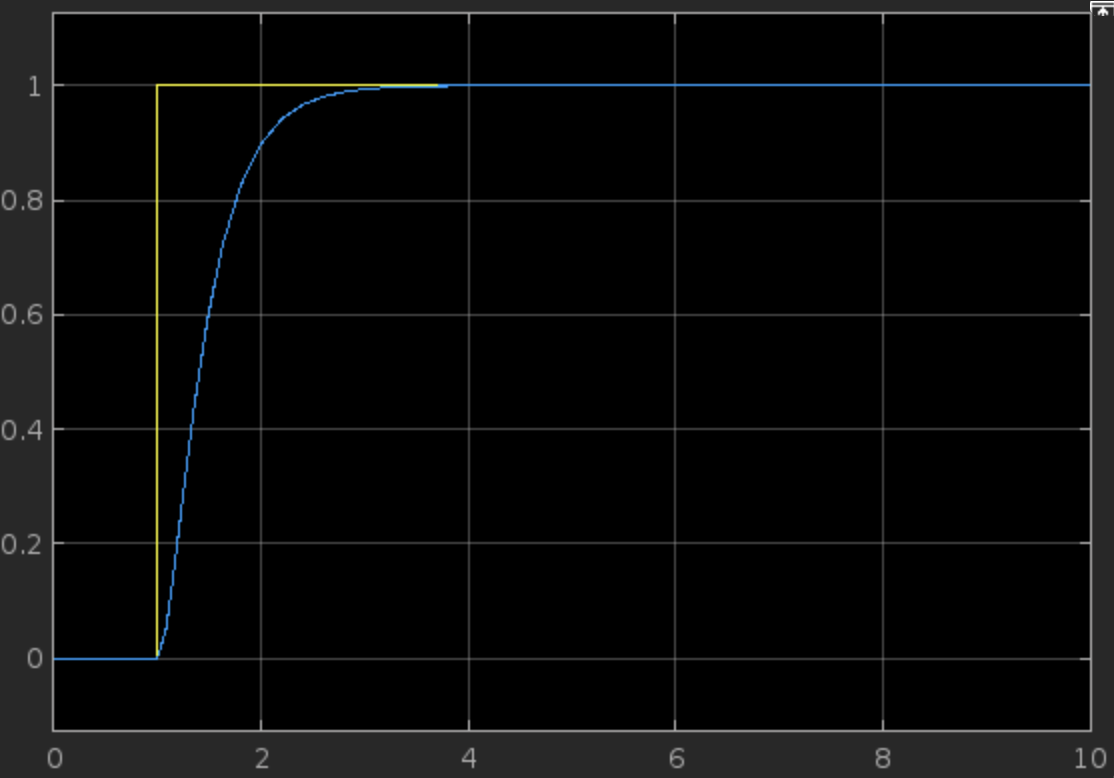
\includegraphics[scale=0.2325, center]{2_b_2_KP_2.png}
					\caption{$K_P = 2$}
					\label{fig6: Graph_KP_2}
				\end{figure}	
\newpage
				\begin{figure}[h]
					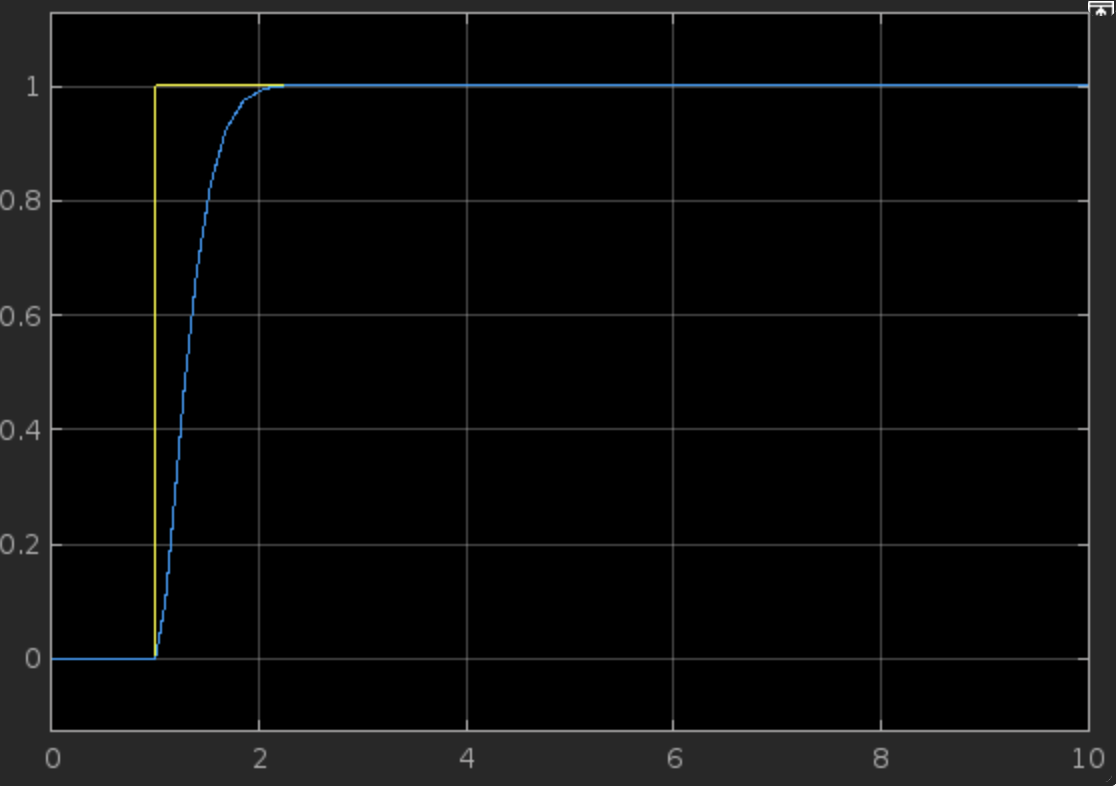
\includegraphics[scale=0.225, center]{2_b_2_KP_3.png}
					\caption{$K_P = 3$}
					\label{fig7: Graph_KP_3}
				\end{figure}
				\begin{figure}[h]
					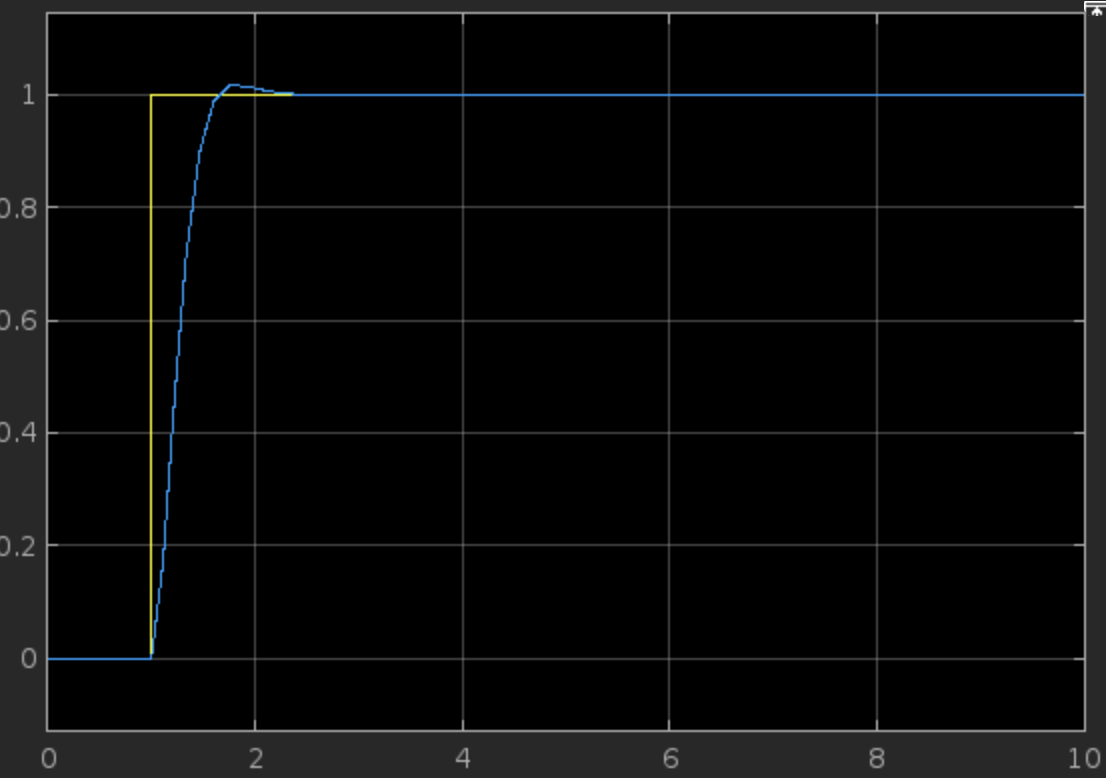
\includegraphics[scale=0.225, center]{2_b_2_KP_4.png}
					\caption{$K_P = 4$}
					\label{fig8: Graph_KP_4}
				\end{figure}
\newpage
				\begin{figure}[h]
					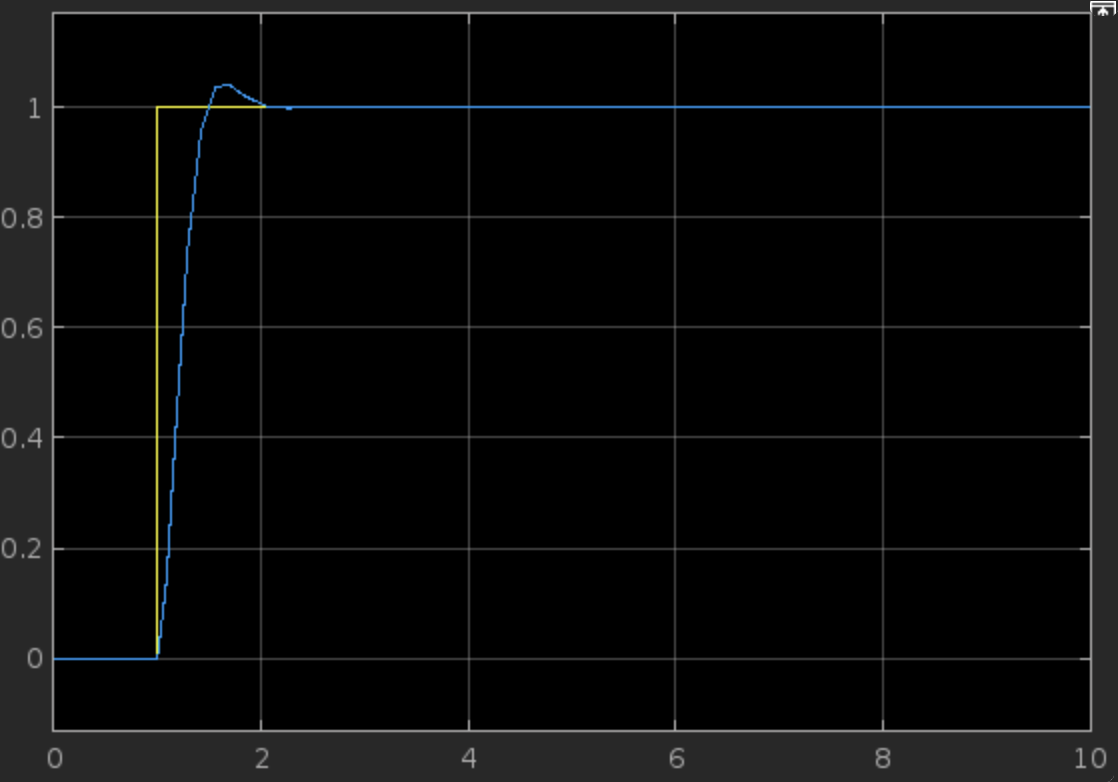
\includegraphics[scale=0.225, center]{2_b_2_KP_5.png}
					\caption{$K_P = 5$}
					\label{fig9: Graph_KP_5}
				\end{figure}
				\begin{figure}[h]
					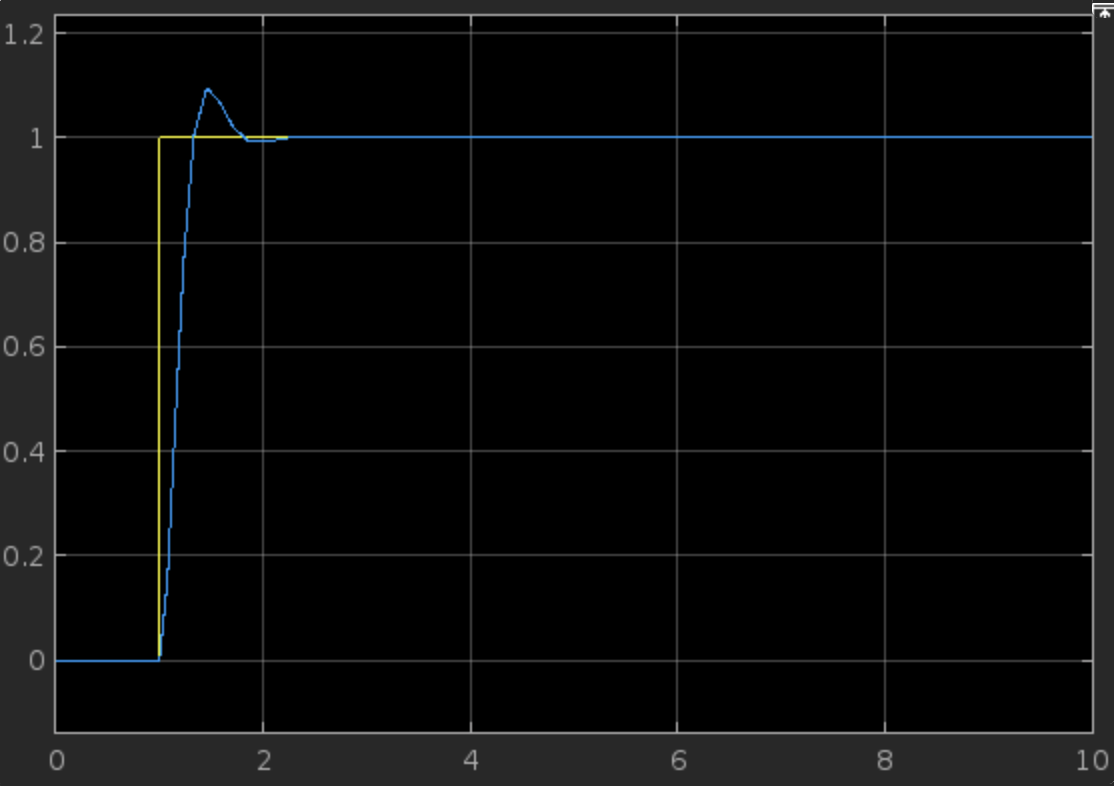
\includegraphics[scale=0.225, center]{2_b_2_KP_7.png}
					\caption{$K_P = 7$}
					\label{fig10: Graph_KP_7}
				\end{figure}
\newpage
				\begin{figure}[h]
					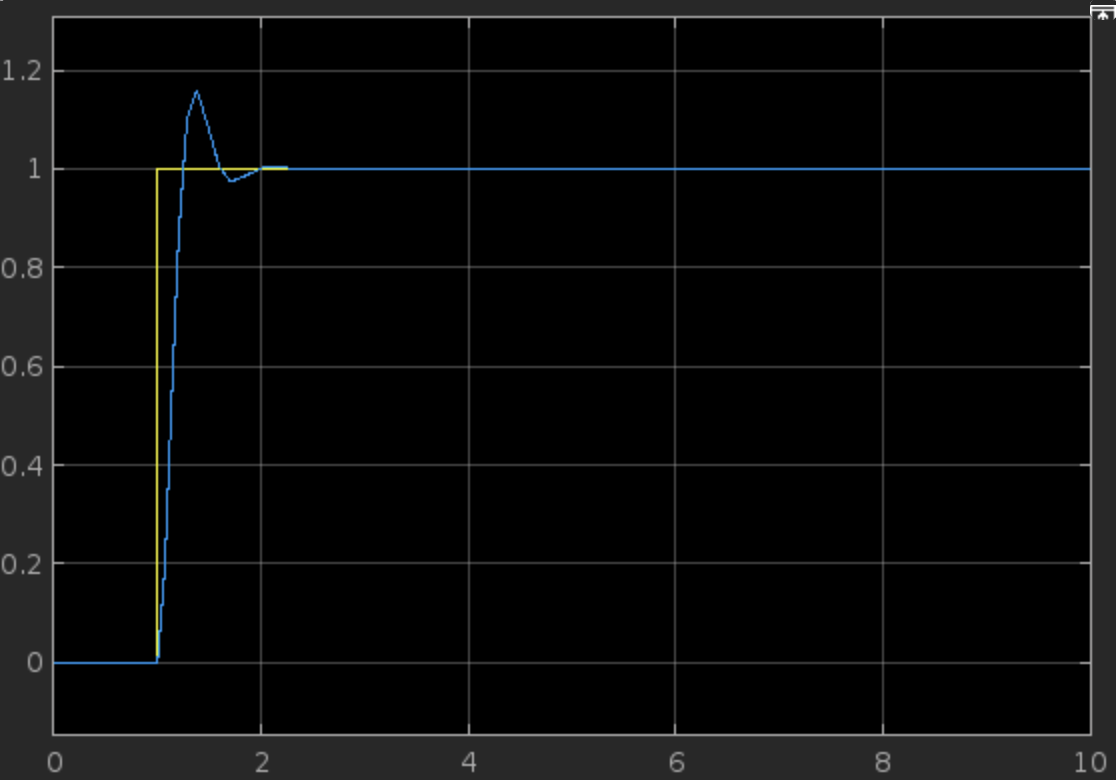
\includegraphics[scale=0.225, center]{2_b_2_KP_10.png}
					\caption{$K_P = 10$}
					\label{fig11: Graph_KP_10}
				\end{figure}
				\begin{figure}[h]
					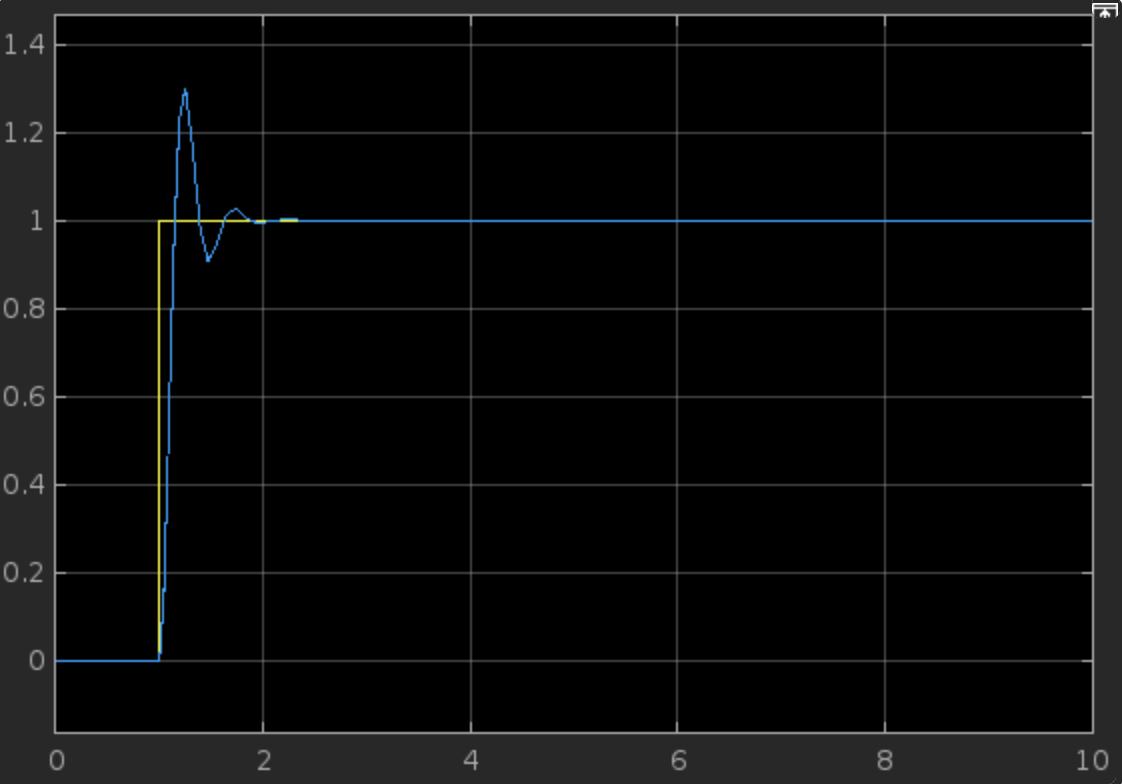
\includegraphics[scale=0.225, center]{2_b_2_KP_20.png}
					\caption{$K_P = 20$}
					\label{fig12: Graph_KP_20}
				\end{figure}
\newpage
				\begin{figure}[h]
					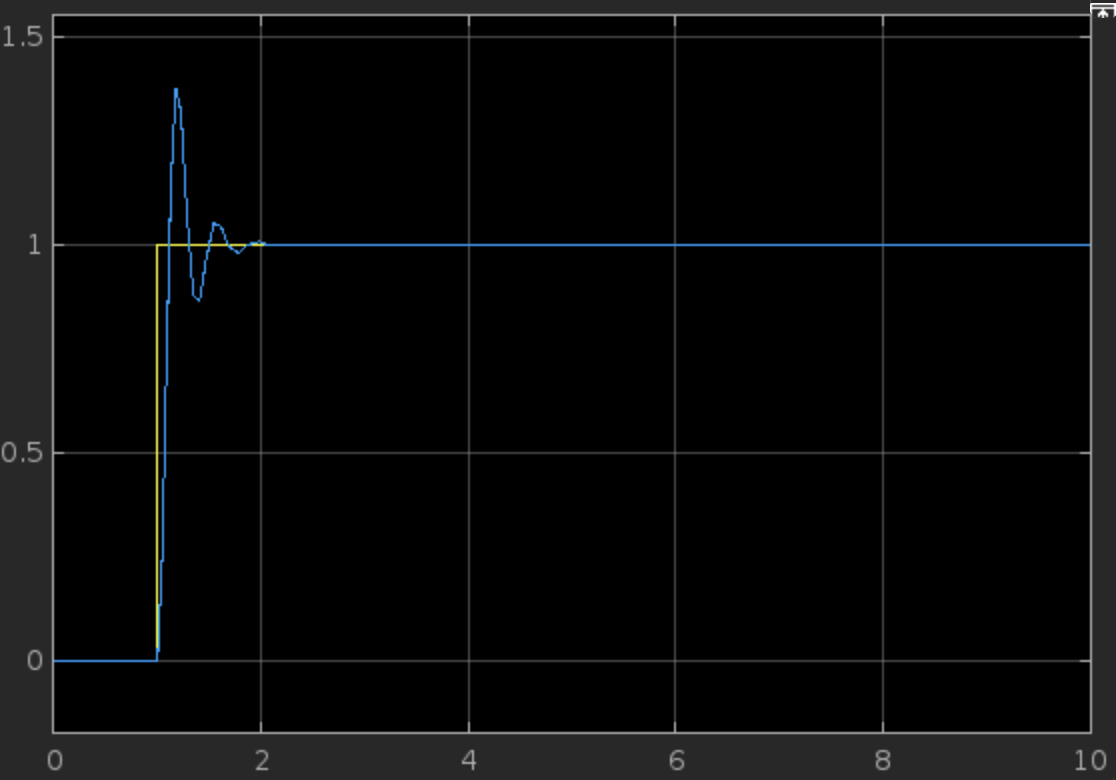
\includegraphics[scale=0.225, center]{2_b_2_KP_30.png}
					\caption{$K_P = 30$}
					\label{fig13: Graph_KP_30}
				\end{figure}
			\subsubsection{$K_{P,opt}$}
				Bei $K_{P,opt}$ handelt es sich um den optimalen Wert für den Faktor. Damit will man erreichen, dass das Signal ein minimales Überschwingen hat. Hier zu sehen in Abb. 4.
				\begin{figure}[h]
					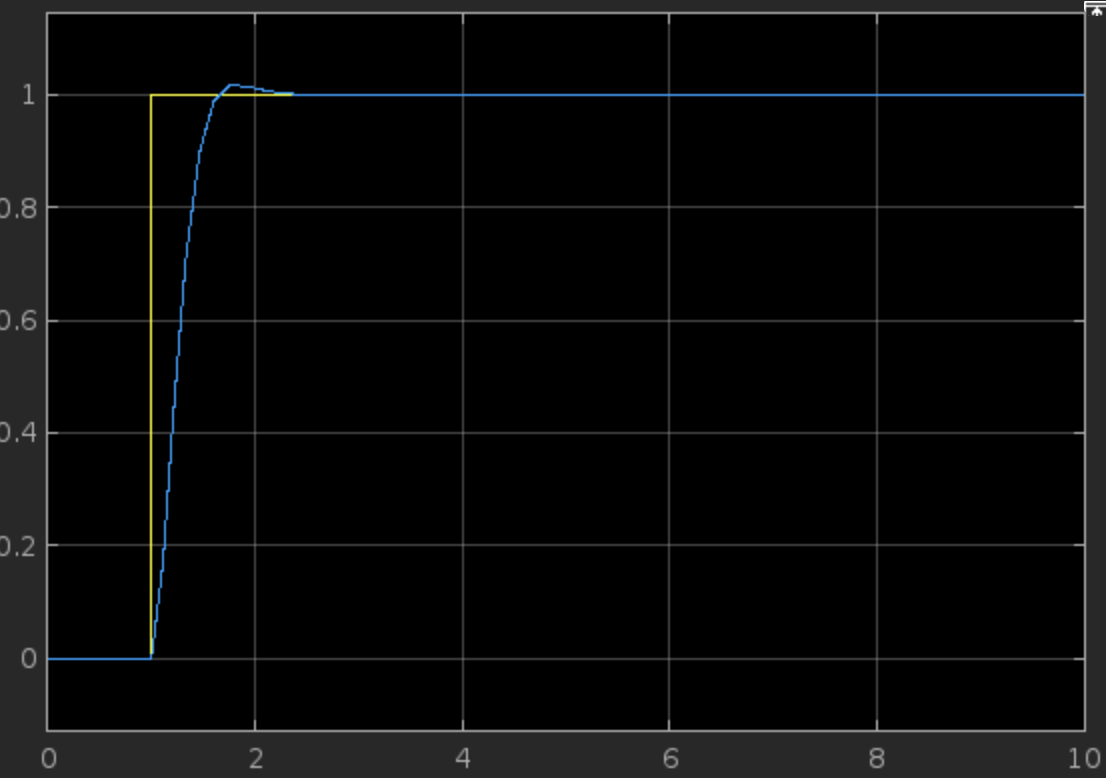
\includegraphics[scale=0.225, center]{2_b_2_KP_4.png}
					\caption{$K_{P,opt} = 4$ mit einem minimalen Überschwinger}
					\label{fig14: Graph_KP_4}
				\end{figure}
\newpage
		\subsection{Lageregelkreis als $PT_2$-Glied}
			\subsubsection{Simulink}
				\begin{figure}[h]
					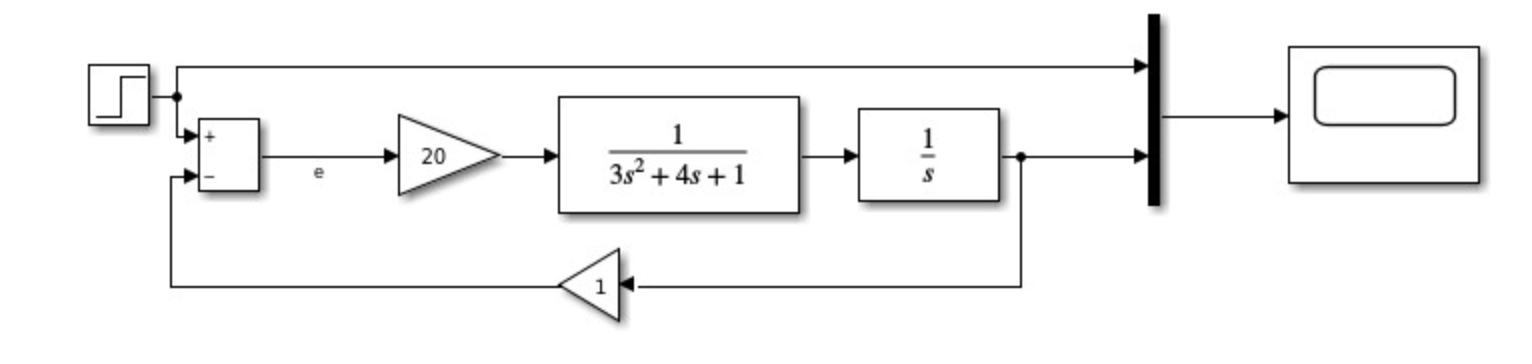
\includegraphics[scale=0.225, center]{2_c_Regelkreis_PT2.png}
					\caption{Lageregelkreis in Simulink als $PT_2$-Glied}
					\label{fig15: Graph_KP_4}
				\end{figure}
			\subsubsection{$K_P$ ermitteln durch probieren}
				\begin{figure}[h]
					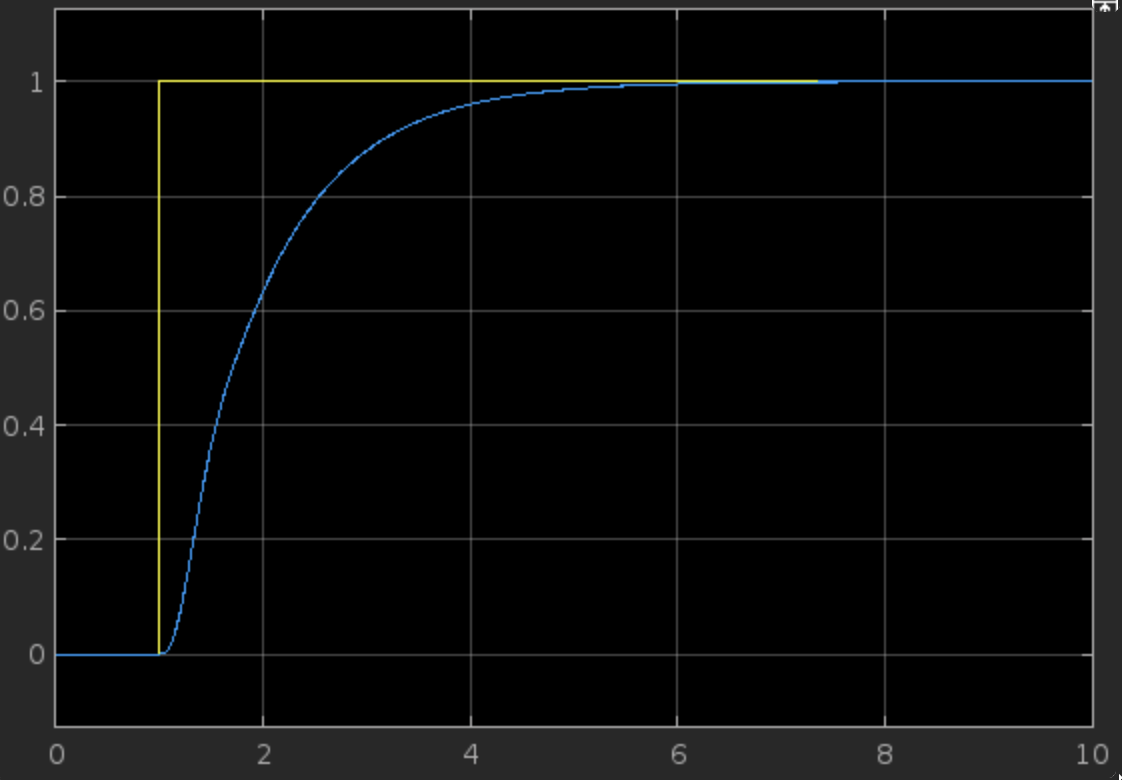
\includegraphics[scale=0.225, center]{2_c_KP_1.png}
					\caption{$K_P = 1$}
					\label{fig16: Graph_c_KP_1}
				\end{figure}				
\newpage
				\begin{figure}[h]
					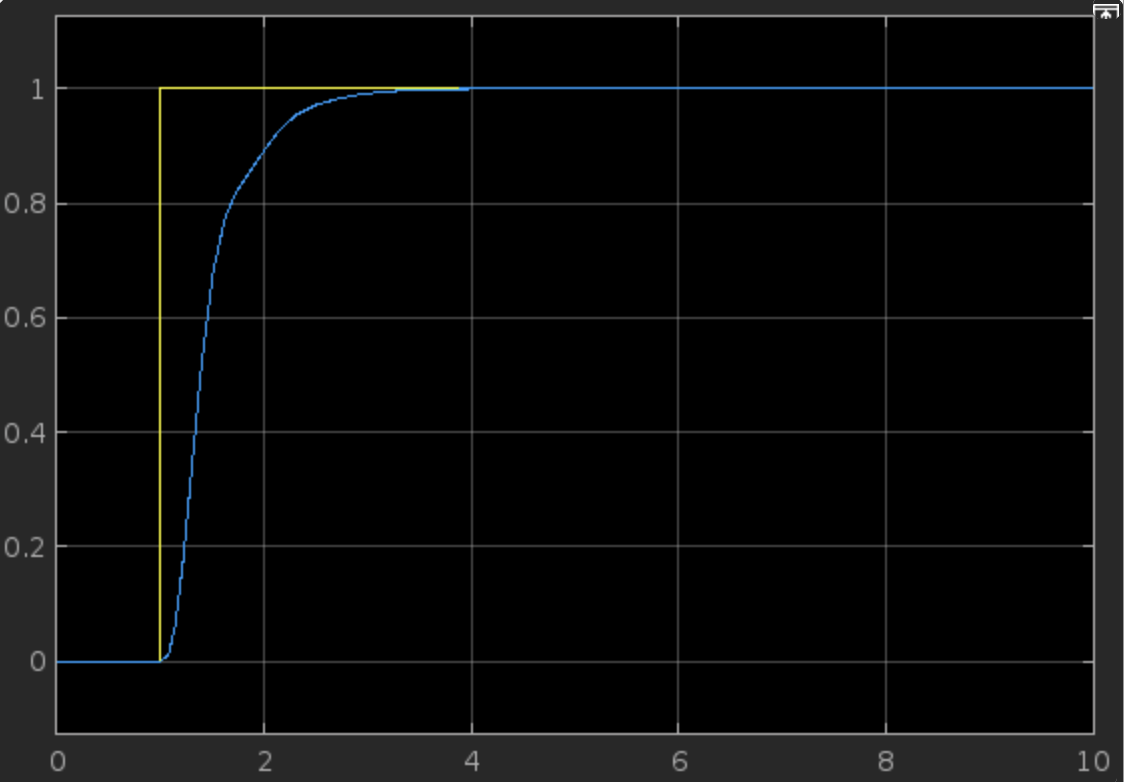
\includegraphics[scale=0.225, center]{2_c_KP_2.png}
					\caption{$K_P = 2$}
					\label{fig17: Graph_c_KP_2}
				\end{figure}				
				\begin{figure}[h]
					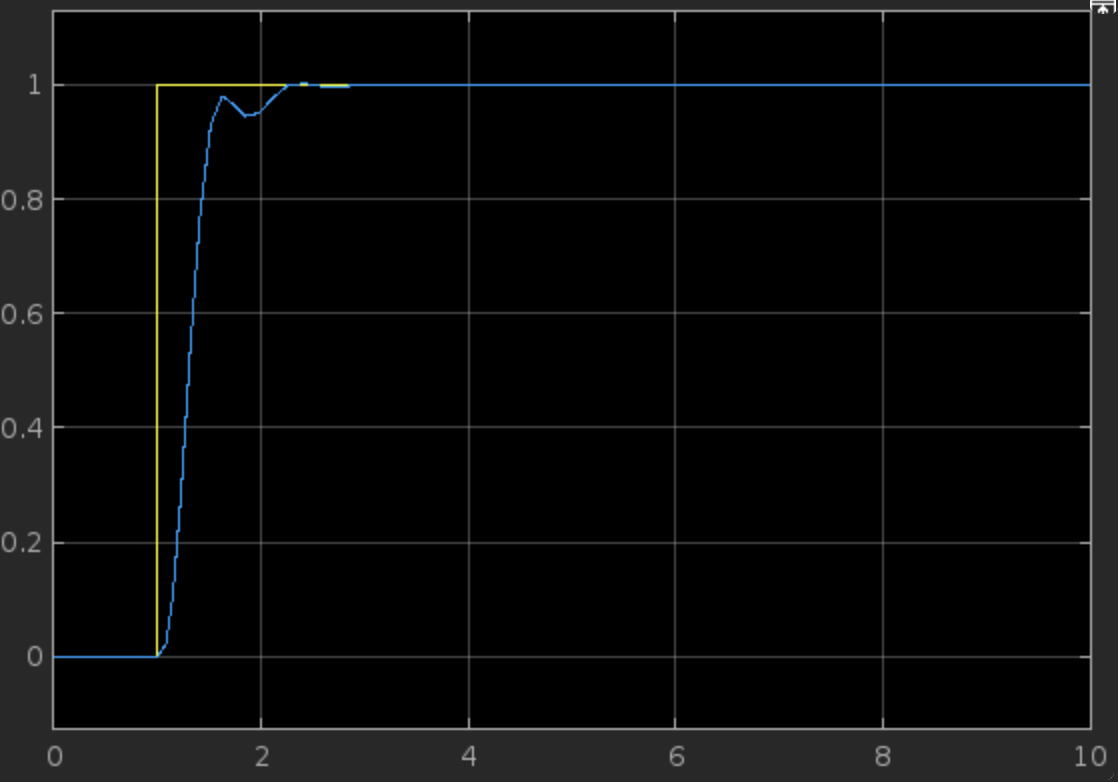
\includegraphics[scale=0.225, center]{2_c_KP_3.png}
					\caption{$K_P = 3$}
					\label{fig18: Graph_c_KP_3}
				\end{figure}					
\newpage
				\begin{figure}[h]
					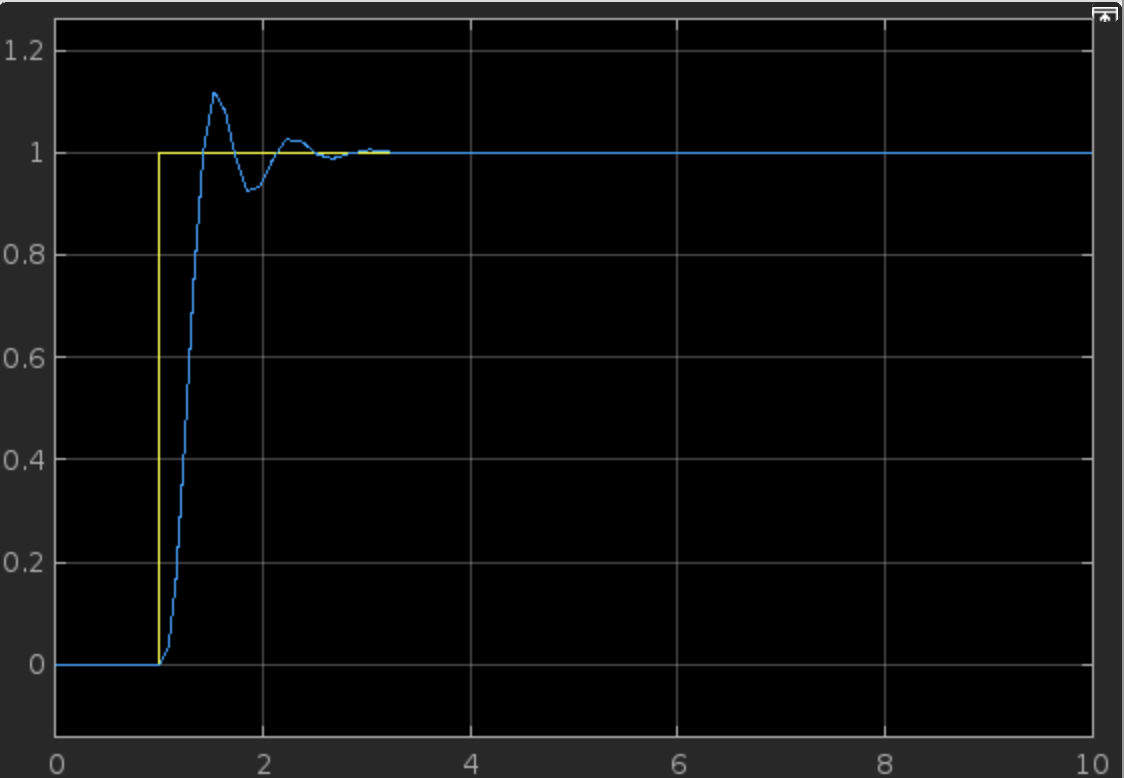
\includegraphics[scale=0.225, center]{2_c_KP_4.png}
					\caption{$K_P = 4$}
					\label{fig19: Graph_c_KP_4}
				\end{figure}				
				\begin{figure}[h]
					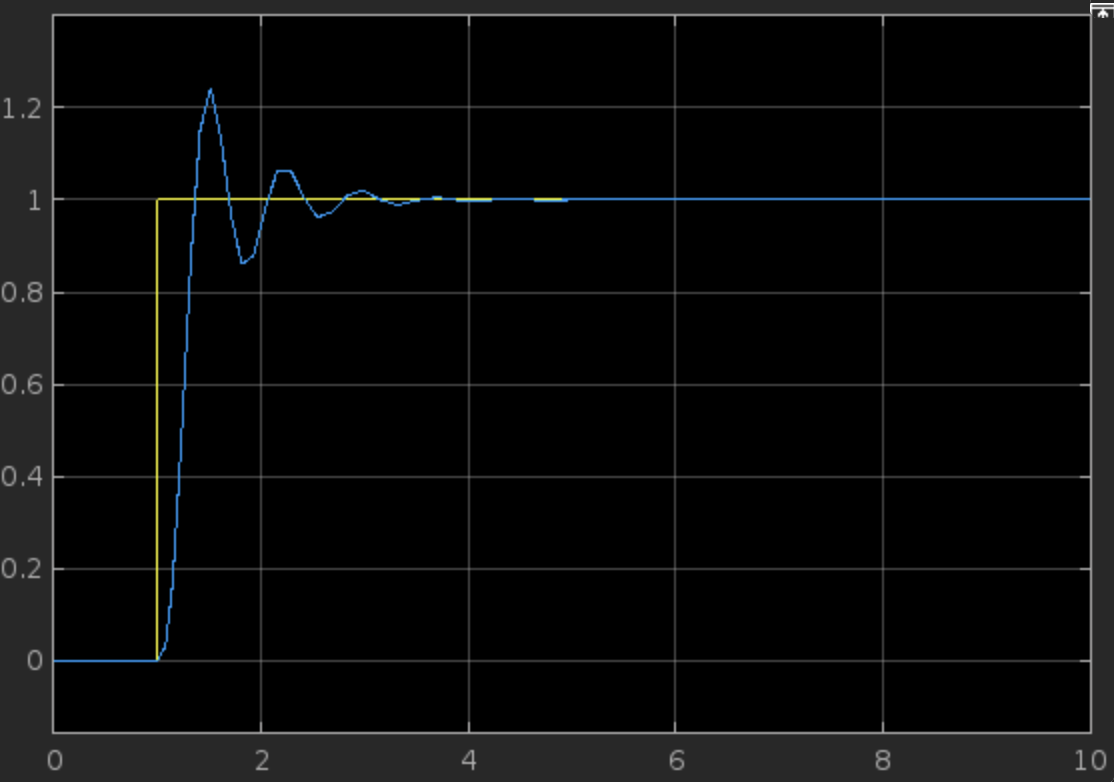
\includegraphics[scale=0.225, center]{2_c_KP_5.png}
					\caption{$K_P = 5$}
					\label{fig20: Graph_c_KP_5}
				\end{figure}	
\newpage
				\begin{figure}[h]
					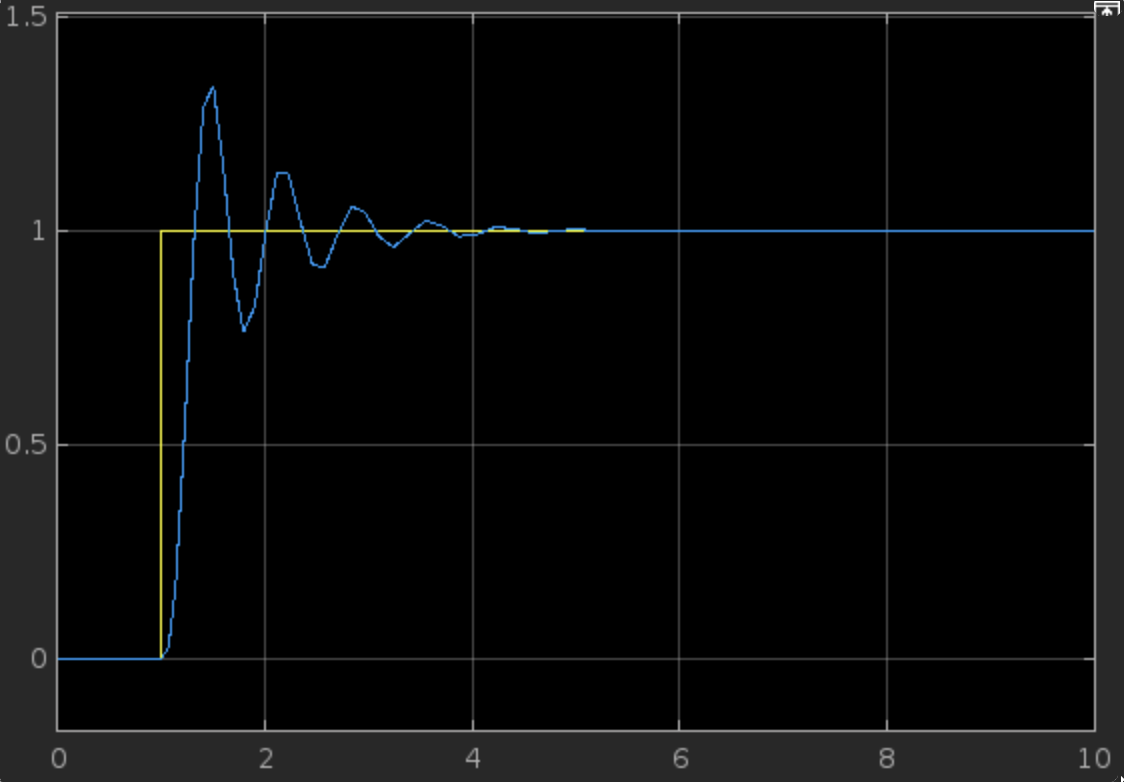
\includegraphics[scale=0.225, center]{2_c_KP_6.png}
					\caption{$K_P = 6$}
					\label{fig21: Graph_c_KP_6}
				\end{figure}			
				\begin{figure}[h]
					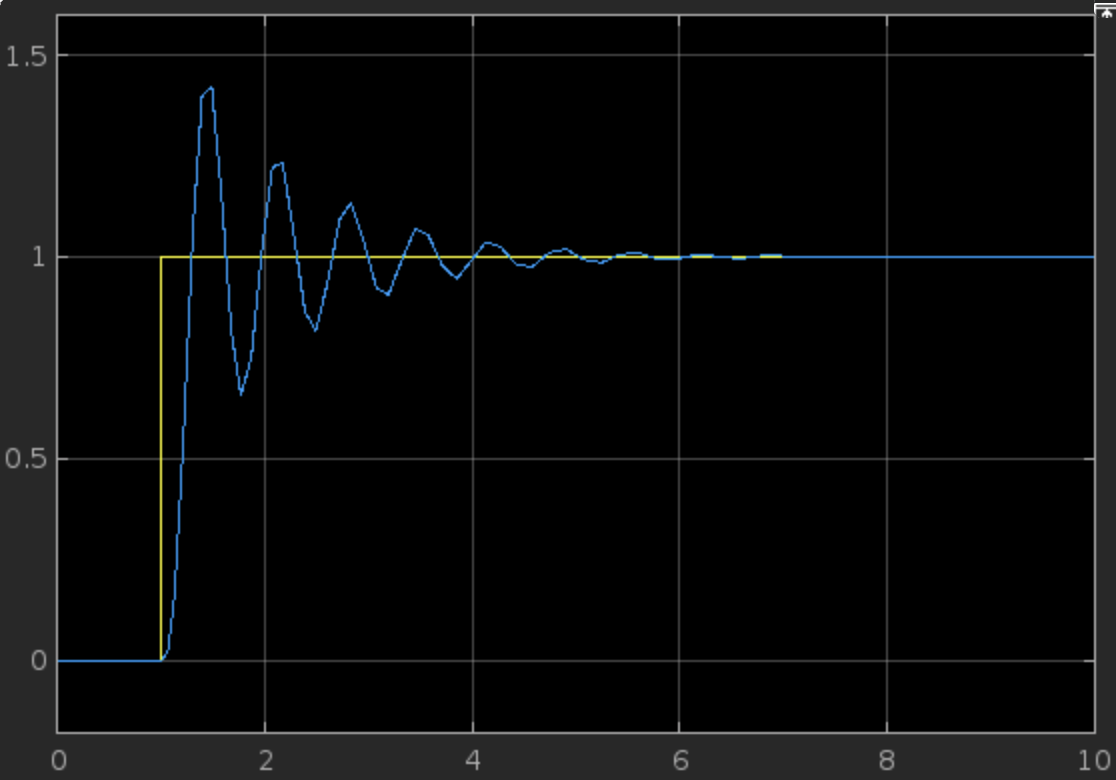
\includegraphics[scale=0.225, center]{2_c_KP_7.png}
					\caption{$K_P = 7$}
					\label{fig22: Graph_c_KP_7}
				\end{figure}		
\newpage
				\begin{figure}[h]
					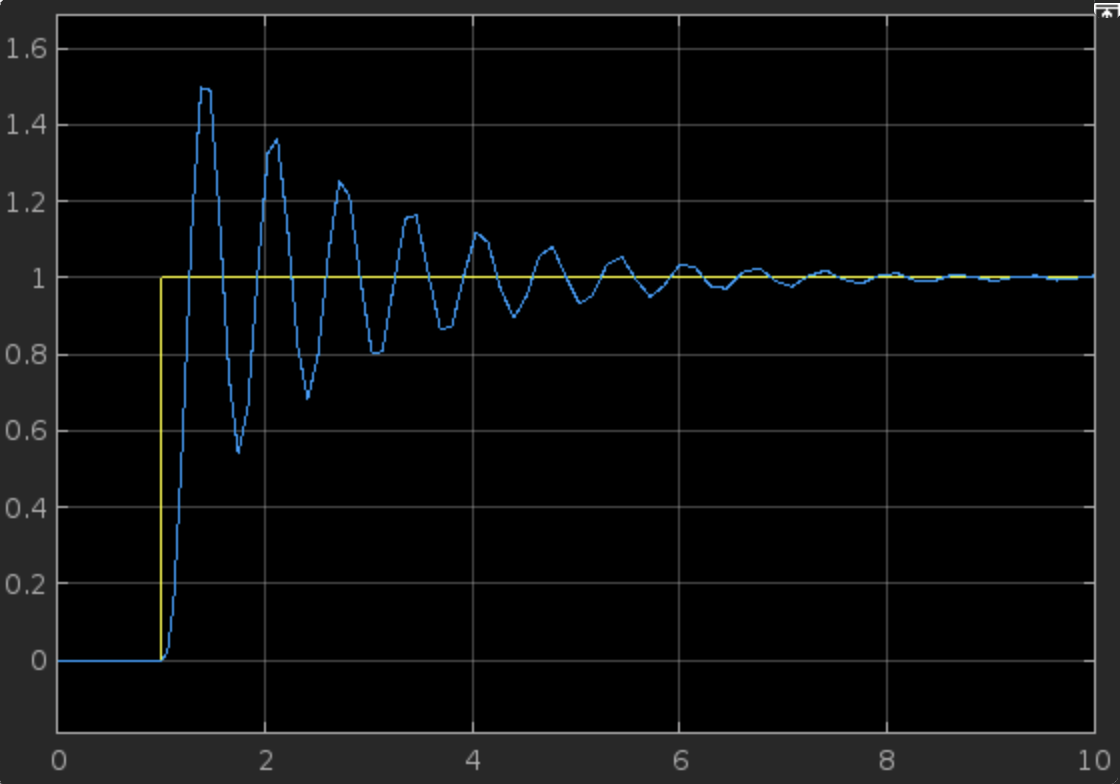
\includegraphics[scale=0.225, center]{2_c_KP_8.png}
					\caption{$K_P = 8$}
					\label{fig23: Graph_c_KP_8}
				\end{figure}				
				\begin{figure}[h]
					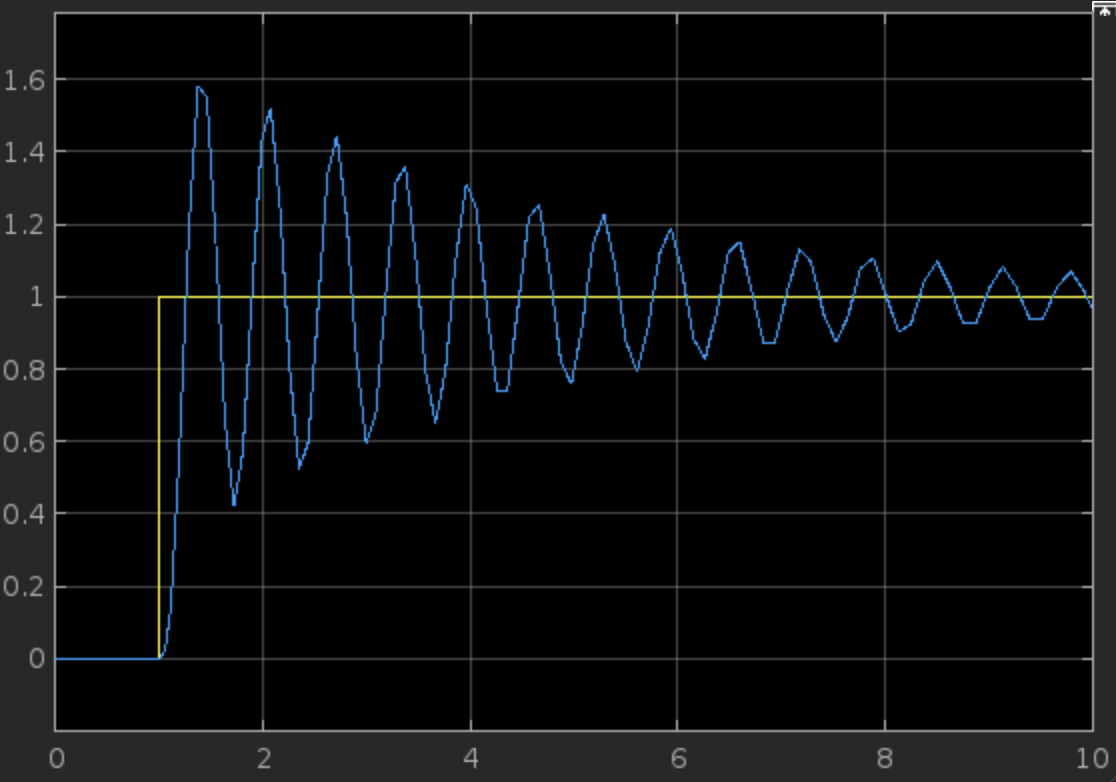
\includegraphics[scale=0.225, center]{2_c_KP_9.png}
					\caption{$K_P = 9$}
					\label{fig24: Graph_c_KP_9}
				\end{figure}	
\newpage
				\begin{figure}[h]
					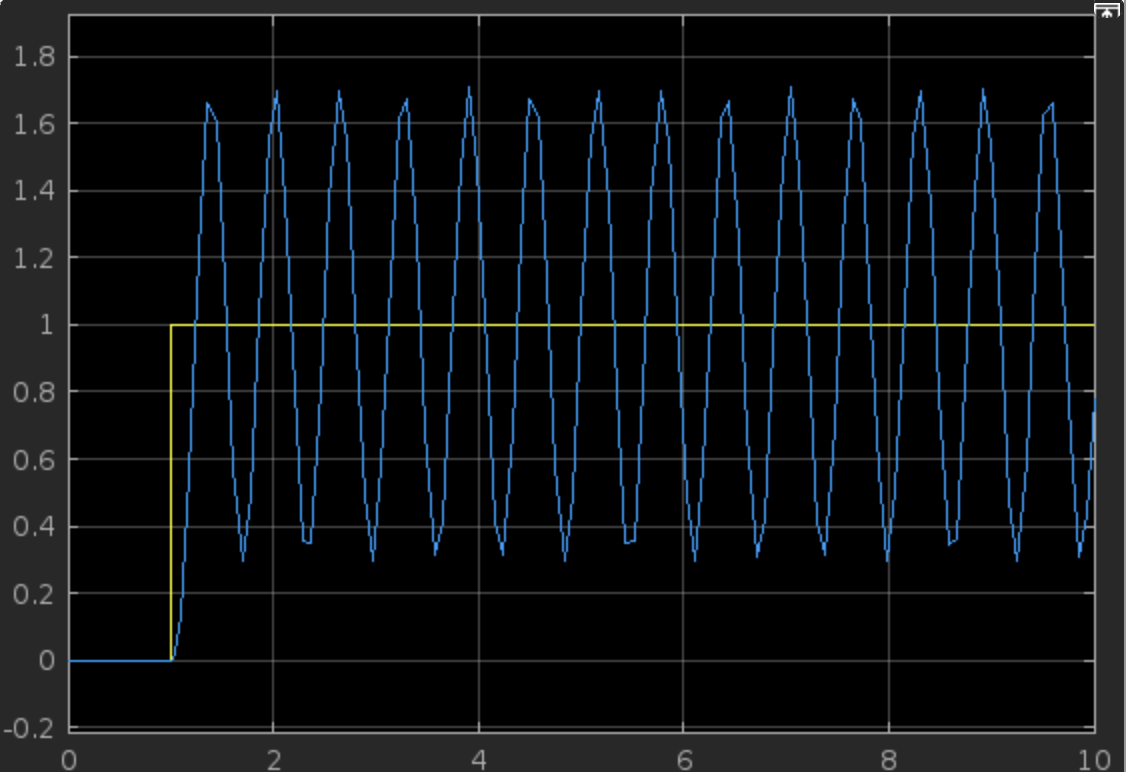
\includegraphics[scale=0.225, center]{2_c_KP_10.png}
					\caption{$K_P = 10$}
					\label{fig25: Graph_c_KP_10}
				\end{figure}				
				\begin{figure}[h]
					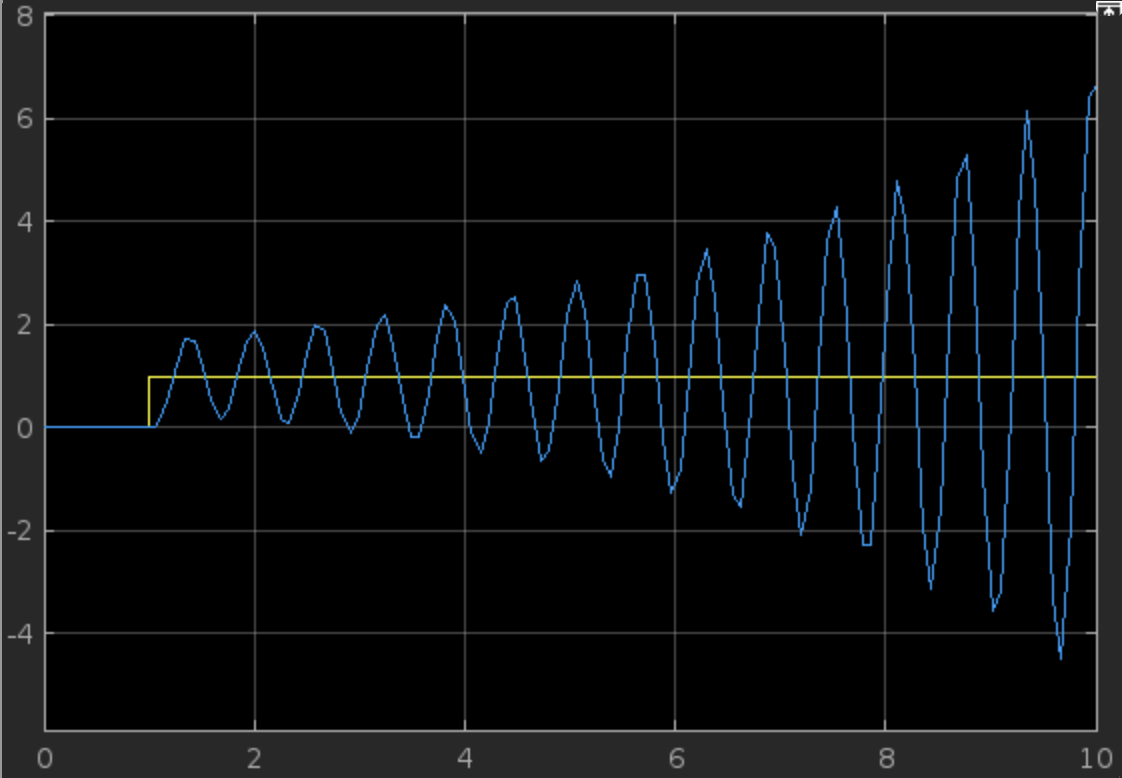
\includegraphics[scale=0.225, center]{2_c_KP_11.png}
					\caption{$K_P = 11$}
					\label{fig26: Graph_c_KP_11}
				\end{figure}	
\newpage
				\begin{figure}[h]
					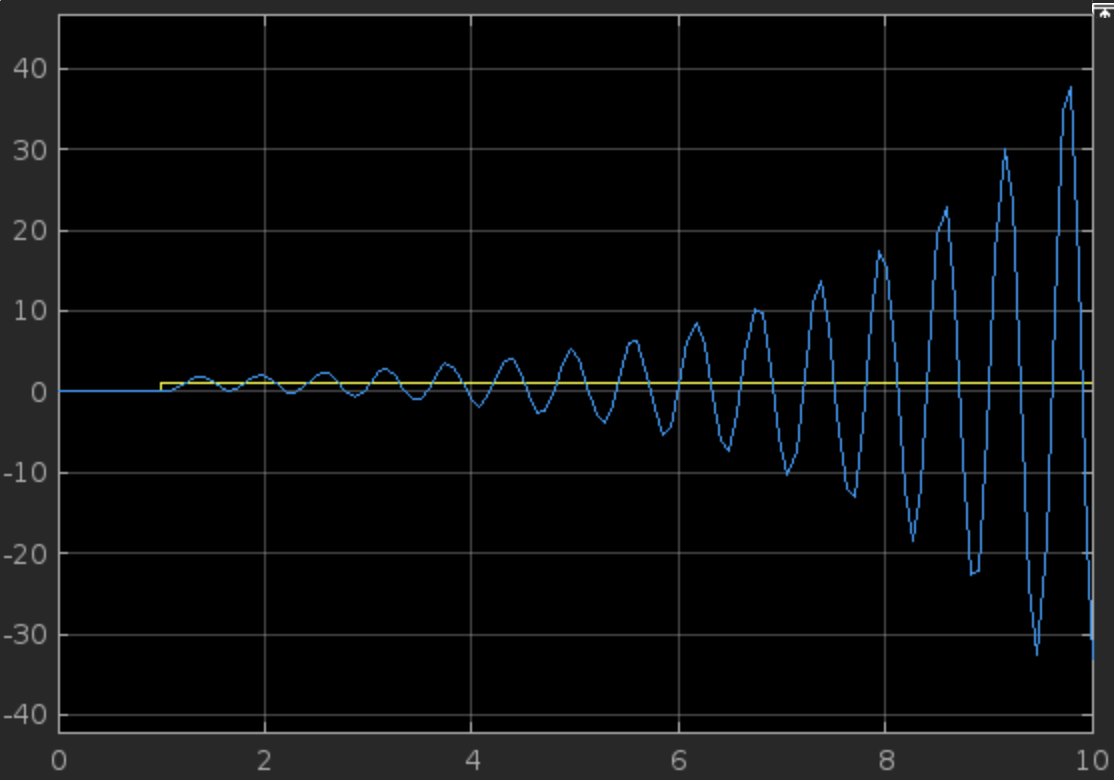
\includegraphics[scale=0.225, center]{2_c_KP_12.png}
					\caption{$K_P = 12$}
					\label{fig27: Graph_c_KP_12}
				\end{figure}				
				\begin{figure}[h]
					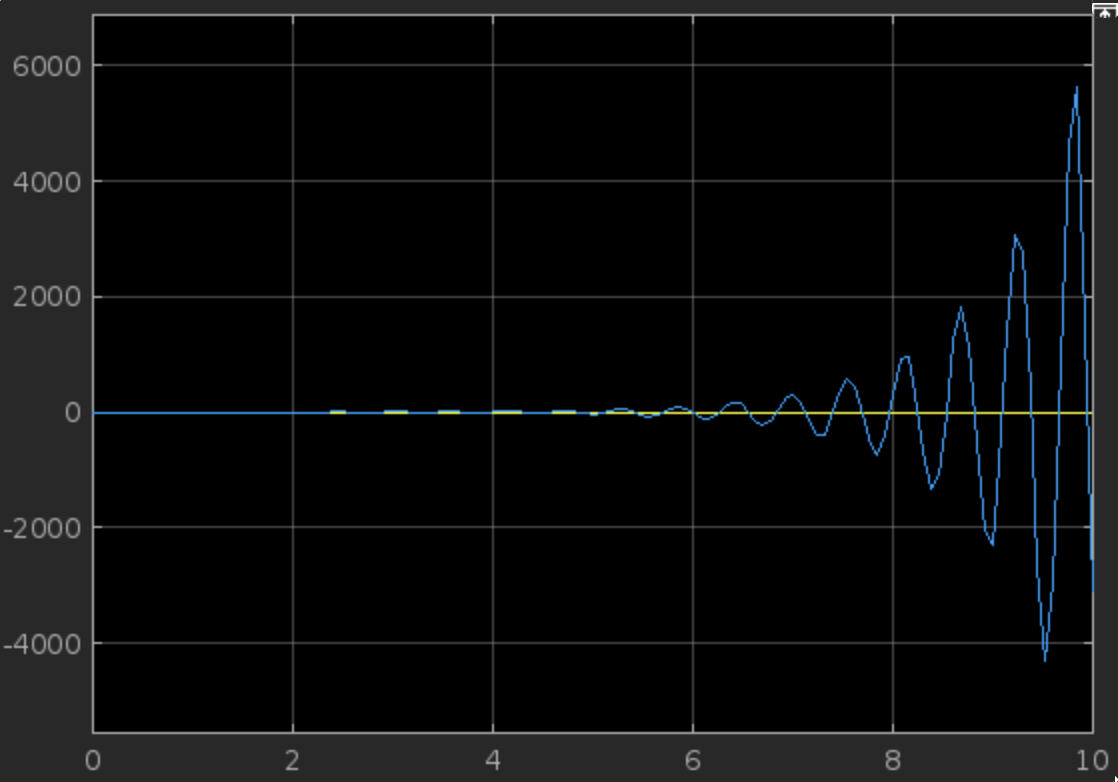
\includegraphics[scale=0.225, center]{2_c_KP_15.png}
					\caption{$K_P = 15$}
					\label{fig28: Graph_c_KP_15}
				\end{figure}	
\newpage
				\begin{figure}[h]
					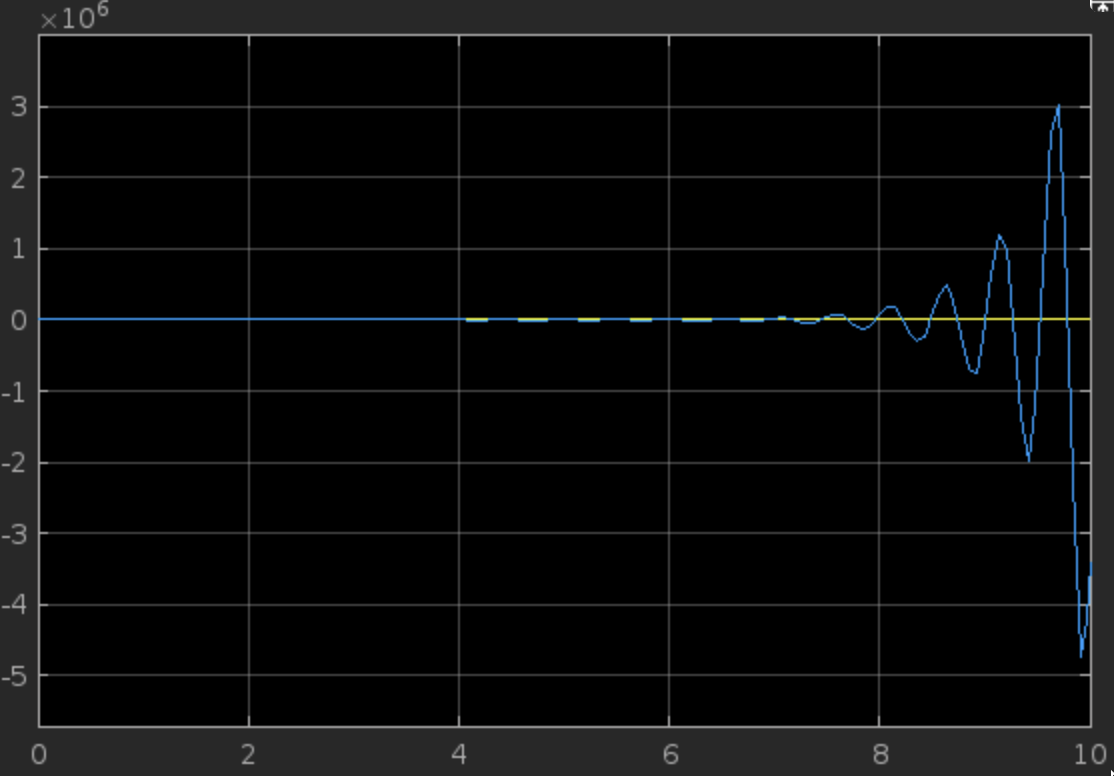
\includegraphics[scale=0.225, center]{2_c_KP_20.png}
					\caption{$K_P = 20$}
					\label{fig29: Graph_c_KP_20}
				\end{figure}				
			\subsubsection{}
				$K_{P,krit}$ verhält sich folgender Maßen:
				\begin{itemize}
					\item bis $K_P = 10$ nimmt das Schwingen ab, zu sehen in den Abb.\ref{fig24: Graph_c_KP_9}
					\item bei $K_P = 10$ ist der optimale Wert erreicht. Das Signal schwingt gleichbleibend auf einer Höhe, zu sehen in Abb.\ref{fig26: Graph_c_KP_11}
					\item über $K_P = 10$ nimmt das Schwingen, zu sehen in Abb.\ref{fig28: Graph_c_KP_15}
				\end{itemize}
				$$K_{P,opt} = \frac{K_{P,krit}}{2} = \frac{10}{2} = 5$$
				$$K_{P,krit} = 2 \cdot K_{P,opt} == 2 \cdot 5 = 10$$
\newpage
	\section{Optimierung nach Zielger/Nichols}
		\subsection{}
			\begin{figure}[h]
				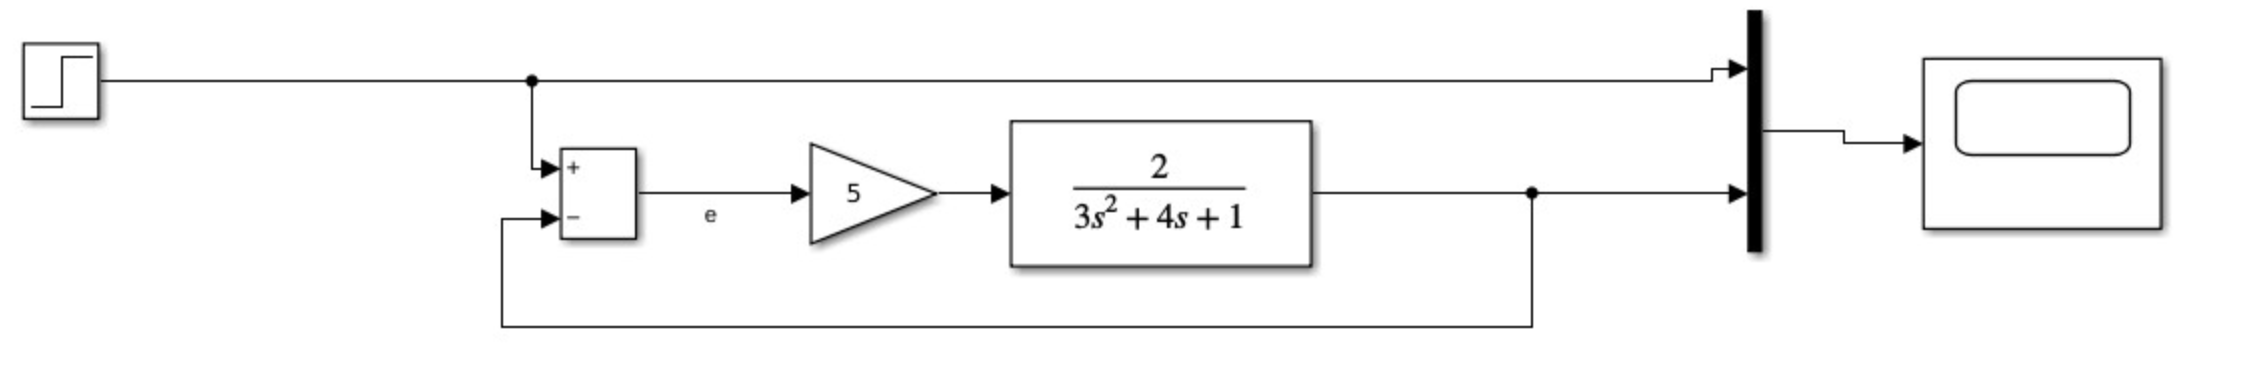
\includegraphics[scale=0.25, center]{3_a_Regelkreis.png}
				\caption{Regelkreis für die Sprungantwort}
				\label{fig30: Regelkreis}
			\end{figure}
			\begin{itemize}
				\item $K_s = 2$
				\item $T_g = 5$
				\item $T_u = 0,5$
			\end{itemize}
		\subsection{Ziegler-Nichols-Einstellkriterium}
			\begin{center}
				\begin{tabular}{ c || c | c | c }
					 Regler & $K_P$ & $T_n$ & $T_v$ \\ 
					 \hline\hline
					 P & $\frac{T_g}{(K_s \cdot T_u}$ &  &  \\  
					 \hline
					 PI & $0.9 \cdot \frac{T_g}{(K_s \cdot T_u}$ & $3.3 \cdot T_u$ &    \\
					 \hline
					 PID & $1.2 \cdot \frac{T_g}{(K_s \cdot T_u)}$ & $2.0 \cdot T_u$ & $0.5 \cdot T_u$
				\end{tabular}
			\end{center}
\vspace{3mm}
			Mit den oben definierten Werten für $K_s$, $T_u$ und $T_v$ bekommt man für die benötigten Zellen der Tabelle, \textit{P} und \textit{PI}, folgende Werte:
			\begin{center}
				\begin{tabular}{ c || c | c | c }
					 Regler & $K_P$ & $T_n$ & $T_v$ \\ 
					 \hline\hline
					 P & $2,08$ &  &  \\  
					 \hline
					 PI & $4,5$ & $1,65$ & 
				\end{tabular}
			\end{center}
\newpage
		\subsection{Blockschaltbild}
		\begin{figure}[h]
			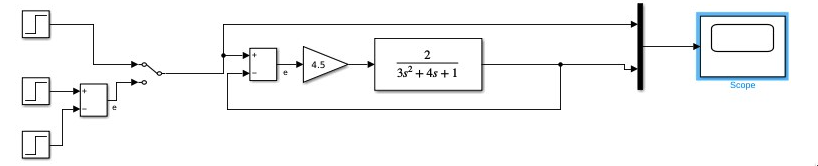
\includegraphics[scale = 0.69, center]{2_3c/3_c_Regelkreis_schalter_oben.png}
			\caption{Schalter in Ausgangsposition.}
			\label{fig31: Blockschaltbild_Ausgangsposition}
		\end{figure}
		Durch Ändern von $K_P$ werden folgende Signalbilder erzeugt:
		\begin{figure}[h]
			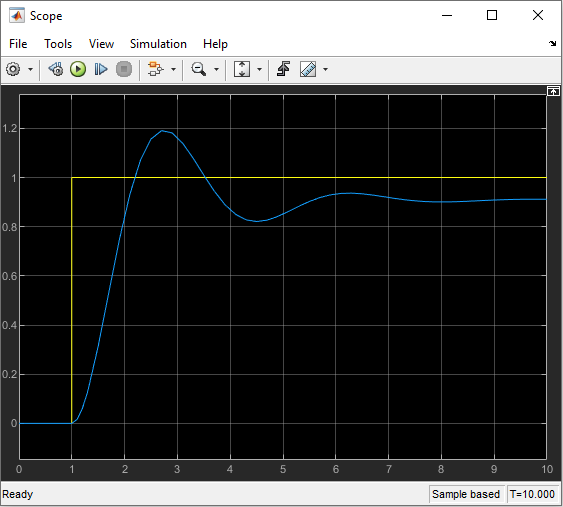
\includegraphics[scale = 0.625, center]{2_3c/5.png}
			\caption{$K_P = 5$}
			\label{fig31: KP_5}
		\end{figure}
\newpage
		\begin{figure}[h]
			\begin{subfigure}{0.5\textwidth}
				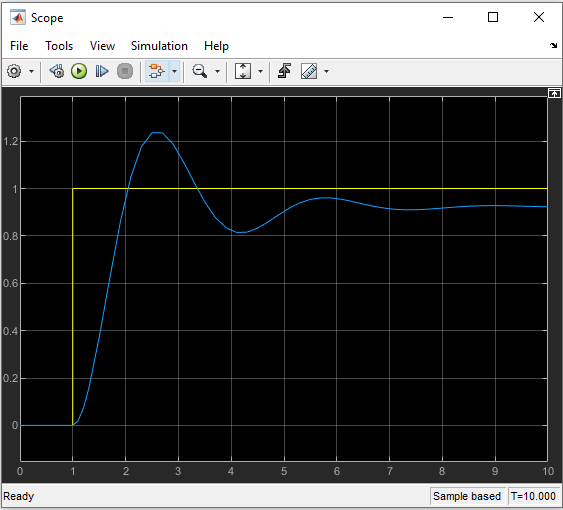
\includegraphics[width=1\linewidth, height=6.5cm]{2_3c/6.png} 
				\caption{$K_P = 6$}
				\label{fig:subim1}
			\end{subfigure}
			\begin{subfigure}{0.5\textwidth}
				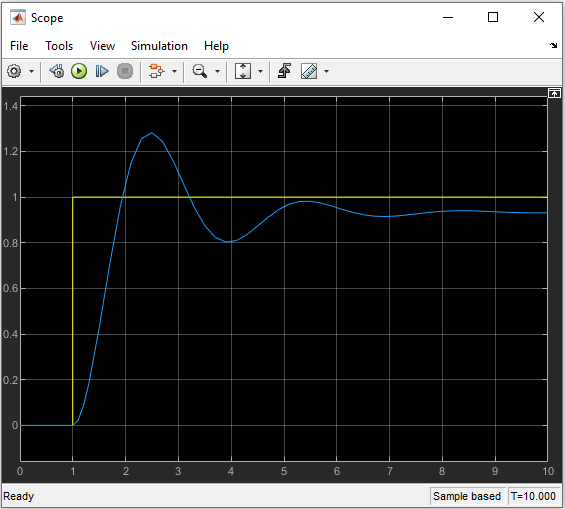
\includegraphics[width=1\linewidth, height=6.5cm]{2_3c/7.png}
				\caption{$K_P = 7$}
				\label{fig:subim2}
			\end{subfigure}
			\begin{subfigure}{0.5\textwidth}
				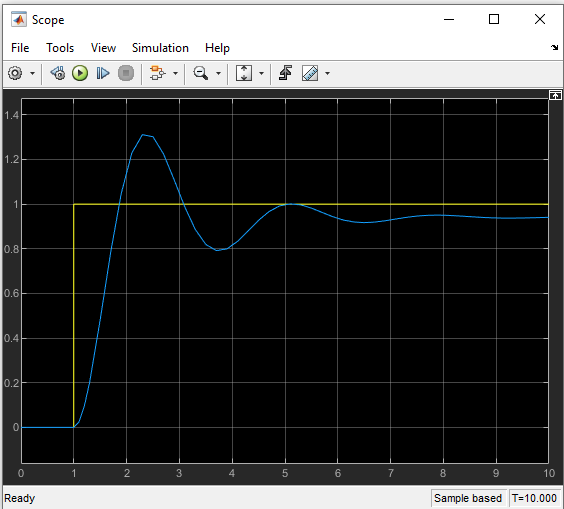
\includegraphics[width=1\linewidth, height=6.5cm]{2_3c/8.png} 
				\caption{$K_P = 8$}
				\label{fig:subim1}
			\end{subfigure}
			\begin{subfigure}{0.5\textwidth}
				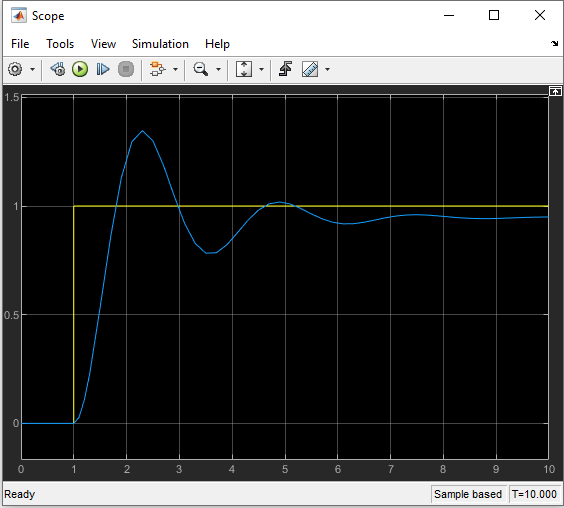
\includegraphics[width=1\linewidth, height=6.5cm]{2_3c/9.png}
				\caption{$K_P = 9$}
				\label{fig:subim2}
			\end{subfigure}
			\label{fig:image2}
		\end{figure}
\newpage
		\begin{figure}[h]
			\begin{subfigure}{0.5\textwidth}
				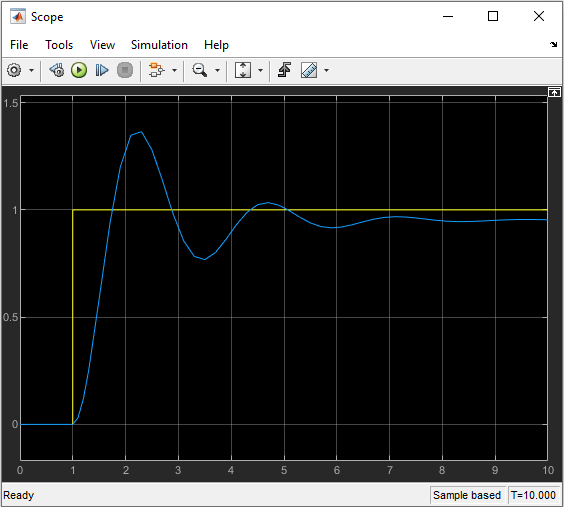
\includegraphics[width=1\linewidth, height=6.5cm]{2_3c/10.png} 
				\caption{$K_P = 10$}
				\label{fig:KP_10}
			\end{subfigure}
			\begin{subfigure}{0.5\textwidth}
				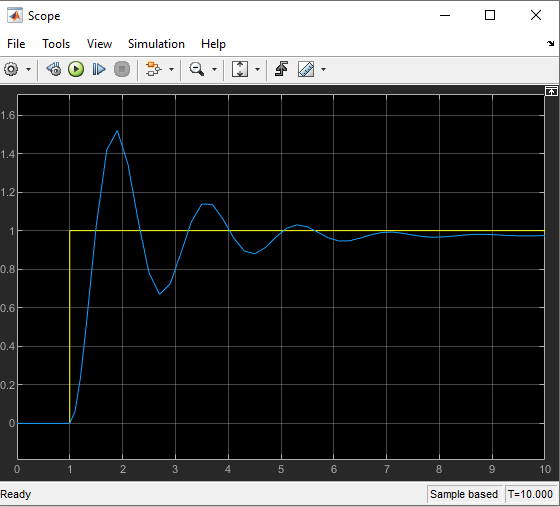
\includegraphics[width=1\linewidth, height=6.5cm]{2_3c/20.png}
				\caption{$K_P = 20$}
				\label{fig:KP_20}
			\end{subfigure}
			\begin{subfigure}{0.5\textwidth}
				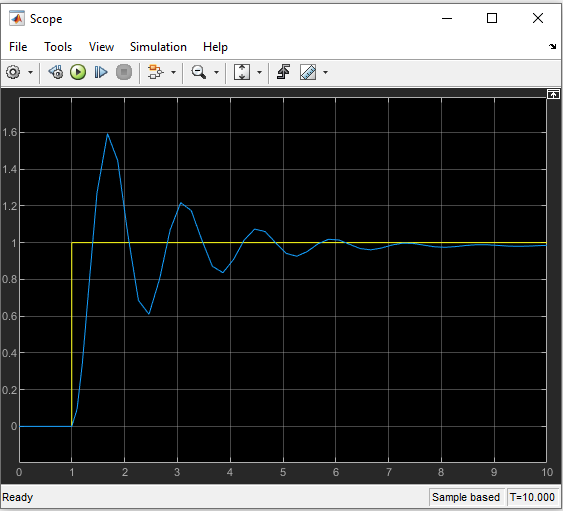
\includegraphics[width=1\linewidth, height=6.5cm]{2_3c/30.png} 
				\caption{$K_P = 30$}
				\label{fig:KP_30}
			\end{subfigure}
			\begin{subfigure}{0.5\textwidth}
				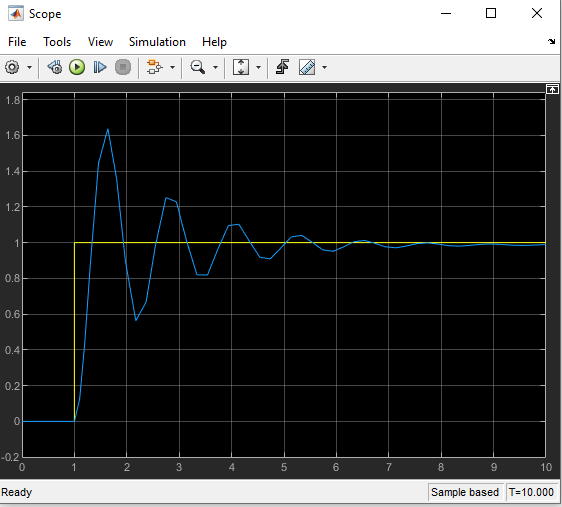
\includegraphics[width=1\linewidth, height=6.5cm]{2_3c/40.png}
				\caption{$K_P = 40$}
				\label{fig:KP_40}
			\end{subfigure}
			\label{fig:image2}
		\end{figure}
\newpage
\newpage
		\begin{figure}[h]
				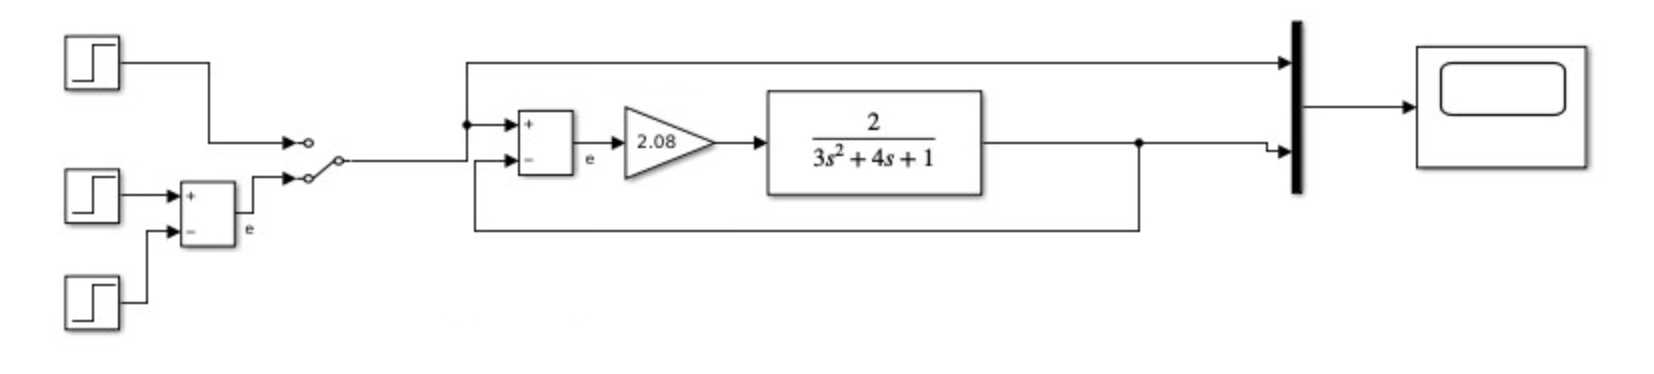
\includegraphics[scale=0.35, center]{2_3c/3_c_Regelkreis.png}
				\caption{Blockschaltbild eines $P$-Regler}
				\label{fig31: Blockschaltbild}
			\end{figure}
			Durch Umlegen des Schalters lassen sich die Sprung- $\epsilon (t)$ und Stoßanregung $\delta (t)$ erzeugen:
\vspace{4mm}
			\begin{figure}[h]
				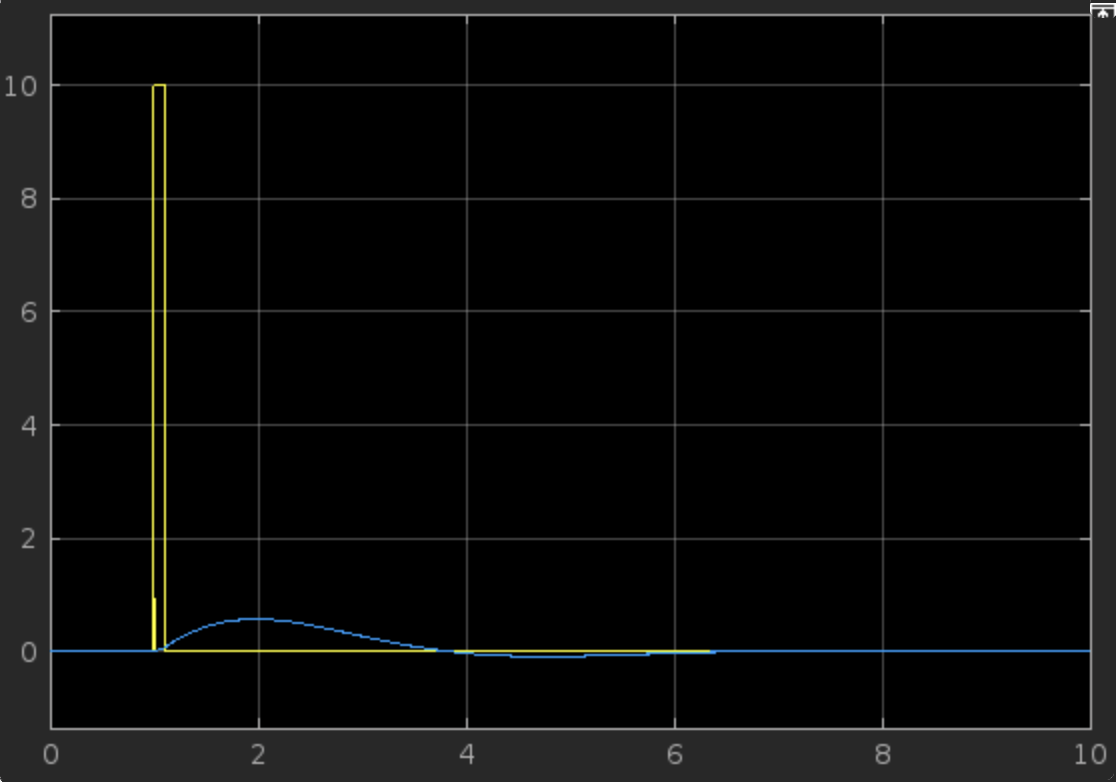
\includegraphics[scale=0.265, center]{Sprungantwort.png}
				\caption{Sprung- in blau und Stoßanregung in gelb; mit dem errechneten $K_P = 2.08$}
				\label{fig32: Sprung. und Stoßantwort}
			\end{figure}
\newpage
			Die Übertragungsfunktion lautet dafür dann:
			$$h(t) = \frac{2.08 \cdot 2}{3s^2 + 4s + 1}$$
			Die Gewichtsfunktion $g(t)$ ist die rücktransformierte der Übertragungsfunktion. \\
			Diese lautet dann :
			$$G(s) = \frac{2.453}{s+} - \frac{0.453}{s+1}$$
\vspace{2mm}	
			$$g_1(t) = 2.453 \cdot e^{-0.33t}$$
\vspace{0mm}
			$$g_2(t) = -0.453 \cdot e^{-t}$$
\vspace{1mm}
			Die gesamte Rücktransformation lautet dann:
			$$g(t) = g_1(t) + g_2(t) = 2.453 \cdot e^{-0.333t} - 0.453 \cdot e^{-t}$$
\vspace{3mm}
			Für einen PI-Regler sieht das ganze folgender Maßen aus:
			\begin{figure}[h]
				\includegraphics[scale=0.5, center]{3_c_PI_Regler_Sprung_Stoß.png}
				\caption{Sprung- in blau und Stoßanregung in gelb; mit dem errechneten $K_P = 1.87$}
				\label{fig32: Sprung. und Stoßantwort}
			\end{figure}	
			
		\subsection{Unterschiede zwischen den Übertragungsfunktionen}
		Ein P-Regler im Regelkreis sorgt für eine begrenzte Steuerungsgenauigkeit. Dabei kann es zu einem Überschwingen, einem langsamen Einschwingverhalten und einer Abweichung von der Sollwert-Position kommen.
		Ein PI-Regler kann das System genauer regeln. Dadurch kann schneller auf Veränderungen reagiert werden, Überschwingen minimal halten und eine stabilere Regelung erreichen.\\
		Die Übergangsfunktion eines PI-Regler ist also schneller und stabiler als bei einem P-Regler.
\newpage
	\section{Regelverhalten von P-, I- und PID-Reglern}
		\subsection{P-Regler}
			Aus der Regelstrecke 
			$$G_S(s) = \frac{K_s}{(1 + T\cdot S)^4}$$
			lässt sich dieser Regelkreis bilden:
			\begin{figure}[h]
				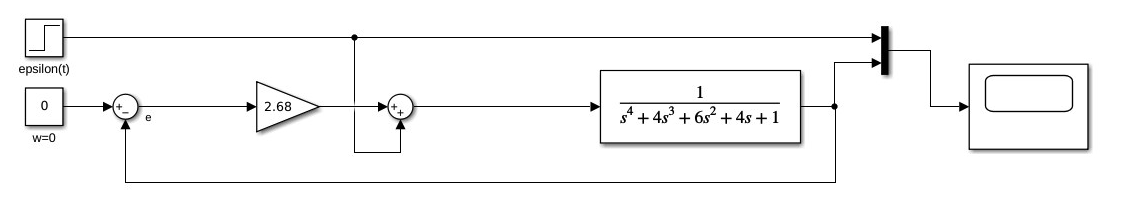
\includegraphics[scale=0.6, center]{4_a_Blockschaltbild.png}
				\caption{Regelkreis mit P-Regler}
				\label{fig33: Blockschaltbild_P_Regler}
			\end{figure}
			Der Graph/das Signal dazu hat folgende Form:
			\begin{figure}[h]
				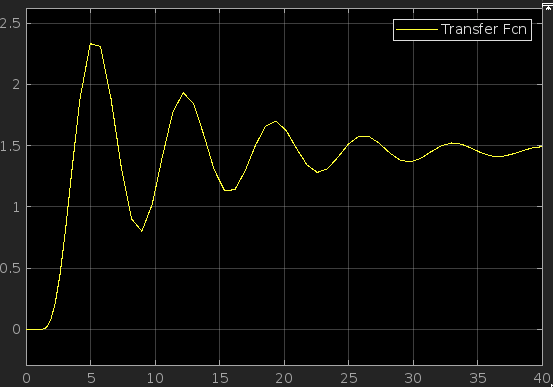
\includegraphics[scale = 0.6, center]{4_a_Graph.png}
				\caption{Das Signal zu oben angegebenen Regelkreis}
				\label{fig34: 4_a_Graph}
			\end{figure}
\newpage
		\subsection{I-Regler}
			Aus der Regelstrecke 
			$$G_S(s) = \frac{K_s}{(1 + T\cdot S)^4}$$
			lässt sich dieser Regelkreis bilden:
			\begin{figure}[h]
				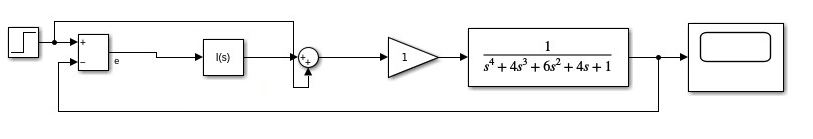
\includegraphics[scale=0.6, center]{4_b_Blockschaltbild.png}
				\caption{Regelkreis mit I-Regler}
				\label{fig35: Blockschaltbild_I_Regler}
			\end{figure}
			Der Graph/das Signal dazu hat folgende Form:
			\begin{figure}[h]
				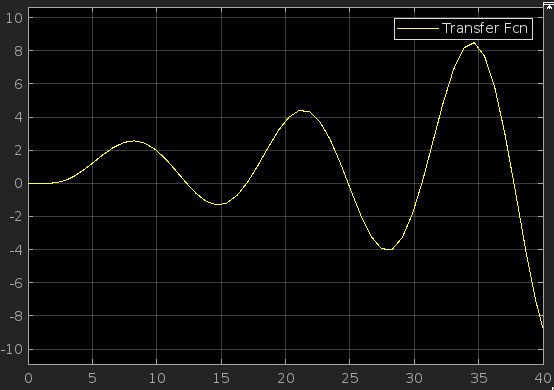
\includegraphics[scale = 0.6, center]{4_b_Graph.png}
				\caption{Das Signal zu oben angegebenen Regelkreis}
				\label{fig36: 4_b_Graph}
			\end{figure}
\newpage
		\subsection{PID-Regler}
			Aus der Regelstrecke 
			$$G_S(s) = \frac{K_s}{(1 T\cdot S)^4}$$
			lässt sich dieser Regelkreis bilden:
			\begin{figure}[h]
				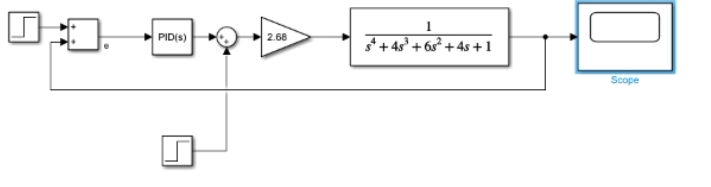
\includegraphics[scale=0.6, center]{4_c_Blockschaltbild.png}
				\caption{Regelkreis mit P-Regler}
				\label{fig37: Blockschaltbild_PID_Regler}
			\end{figure}
			Der Graph/das Signal dazu hat folgende Form:
			\begin{figure}[h]
				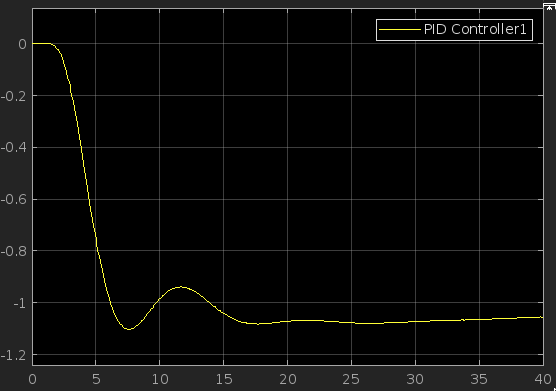
\includegraphics[scale = 0.6, center]{4_c_Graph.png}
				\caption{Das Signal zu oben angegebenen Regelkreis}
				\label{fig38: 4_c_Graph}
			\end{figure}
\newpage
		\subsection{Störübertragungsfunktionen}
			Der Zusammengeführte Regelkreis:
			\begin{figure}[h]
				\includegraphics[scale = 0.4, center]{4_d_Blockschaltbild_alle_zusammen.png}
				\caption{Regelkreis der Zusammengeführten Funktionen aus b), c) un d).}
				\label{fig37:4_d_alle_Regelkreise}
			\end{figure}
			\begin{figure}[h]
				\includegraphics[scale = 0.45, center]{4_d_alle_Graphen.png}
				\caption{Alle Graphen zusammen in ein Bild.}
				\label{fig37:4_d_alle_Regelkreise}
			\end{figure}
				
				
				
				
				
\end{document}